\documentclass[12pt,a4paper]{report}

% ============================================================
% UAB MSc Thesis, modular language-guided NAO interaction stack
% ============================================================

\usepackage[utf8]{inputenc}
\usepackage[T1]{fontenc}
\usepackage[a4paper,margin=22mm,headheight=15pt]{geometry}
\usepackage{setspace}
\usepackage{graphicx}
\usepackage{xcolor}
\usepackage{amsmath,amssymb,mathtools}
\usepackage{enumitem}
\usepackage{booktabs}
\usepackage{float}
\usepackage{array}
\usepackage{longtable}
\usepackage{caption}
\usepackage{subcaption}
\usepackage{tabularx}
\usepackage{csquotes}
\usepackage{url}
\usepackage[toc]{appendix}
\usepackage[section]{placeins}
\usepackage{pdflscape}
\usepackage{ragged2e}
\usepackage{microtype}
\usepackage{needspace}
\usepackage{pgfplots}
\pgfplotsset{compat=1.18}
\usepackage{tikz}
\usetikzlibrary{arrows.meta, positioning, shapes.geometric, shapes.multipart, shadows, fit, backgrounds, calc}
\usepackage{listings}
\usepackage{fancyhdr}
\usepackage[colorlinks=true, linkcolor=black, citecolor=blue, urlcolor=blue]{hyperref}
\hypersetup{
  pdftitle={Design, Integration, and Validation of a Modular Language-Model-Enabled Interaction and Execution Stack for the NAO Robot},
  pdfauthor={Juan David Bendek Williamson},
  pdfsubject={Modular language-guided human-robot interaction and execution on NAO}
}
\usepackage[
  backend=biber,
  style=authoryear,
  maxcitenames=1,
  mincitenames=1,
  uniquelist=false,
  uniquename=false,
  maxbibnames=99
]{biblatex}

\AtEveryCitekey{%
  \defcounter{maxnames}{1}%
  \defcounter{minnames}{1}%
}
\addbibresource{bibliography.bib}

\graphicspath{{images/}}

% ---- Header / footer ----
\pagestyle{fancy}
\fancyhf{}
\renewcommand{\chaptermark}[1]{\markboth{#1}{#1}}
\fancyhead[L]{\nouppercase{\leftmark}}
\fancyhead[R]{Juan David Bendek Williamson}
\fancyfoot[C]{\thepage}

% ---- Paragraph and list spacing ----
\setstretch{1.15}
\setlength{\parskip}{6pt}
\setlength{\parindent}{0pt}
\setlist[itemize]{topsep=3pt,itemsep=2pt,parsep=0pt}
\setlist[enumerate]{topsep=3pt,itemsep=2pt,parsep=0pt}

% ---- Code blocks ----
\lstdefinestyle{sharedCode}{
  basicstyle=\ttfamily\small,
  backgroundcolor=\color{gray!5},
  frame=single,
  numbers=left,
  numberstyle=\tiny\color{gray},
  keywordstyle=\color{blue!70!black},
  commentstyle=\color{gray!80!black},
  stringstyle=\color{green!40!black},
  showstringspaces=false,
  breaklines=true,
  tabsize=2
}
\lstdefinestyle{jsonStyle}{
  basicstyle=\ttfamily\small,
  backgroundcolor=\color{gray!5},
  frame=single,
  numbers=left,
  numberstyle=\tiny\color{gray},
  showstringspaces=false,
  breaklines=true
}
\lstdefinestyle{pythonStyle}{
  language=Python,
  basicstyle=\ttfamily\small,
  backgroundcolor=\color{gray!5},
  frame=single,
  numbers=left,
  numberstyle=\tiny\color{gray},
  keywordstyle=\color{blue!70!black},
  commentstyle=\color{gray!80!black},
  stringstyle=\color{green!40!black},
  showstringspaces=false,
  breaklines=true
}
\lstset{style=sharedCode}

% ---- Colours and commands ----
\definecolor{uabgreen}{RGB}{0,128,64}
\definecolor{lightblue}{RGB}{232,242,255}
\definecolor{lightgreen}{RGB}{235,249,240}
\definecolor{lightorange}{RGB}{255,245,230}
\definecolor{lightgraybox}{RGB}{247,247,247}
\DeclareRobustCommand{\code}[1]{\texttt{\detokenize{#1}}}

\begin{document}
\pagenumbering{roman}

\begin{titlepage}
\centering

\includegraphics[width=0.58\textwidth]{images/uab_logo-gs.png}\\[0.2cm]
{\fontfamily{qhv}\selectfont
\large\textbf{Faculty of Science}
}\\[2.2cm]

\hrule
\vspace{0.9cm}
{\LARGE Design, Integration, and Validation of a Modular Language-Model-Enabled Interaction and Execution Stack for the NAO Robot}\\[8mm]
\hrule
\vspace{18mm}

{\Large\textbf{Juan David Bendek Williamson}}\\[2.3cm]

\large{Supervised by Raquel Ros}\\[0.6cm]
\large{Institution / Lab: IIIA-CSIC / Universitat Aut\`onoma de Barcelona}\\[1.8cm]

\large\textit{Thesis submitted as a requirement for the degree of\\ MSc in Modelling for Science \& Engineering}\\

\vfill
\large{Academic year: 2025--2026}\\[2mm]
Date: \today\\[3mm]
\end{titlepage}

\clearpage
\chapter*{Abstract}
\addcontentsline{toc}{chapter}{Abstract}
\markboth{Abstract}{Abstract}

Large language models have shown strong potential for instruction understanding and high-level reasoning in human-robot interaction. Their integration into a robot nevertheless requires more than a planner call: dialogue state, symbolic grounding, capability descriptions, execution admission, robot-facing skills, feedback, and user-facing reporting must remain coherent across a distributed runtime. This thesis presents the design, integration, and validation of a modular language-model-enabled interaction and execution stack for the NAO robot.

The system separates dialogue management, semantic routing, symbolic grounding, task planning, deterministic orchestration, and skill execution. A chatbot interprets each turn and selects a conversational, knowledge, or execution route. A planner generates structured plans over a reviewed skill registry, while an orchestrator admits requests, validates plans, dispatches real or simulated skills, and returns typed execution feedback. A knowledge and perception path provides compact grounded context without allowing planning-time state to stand in for execution evidence.

The contribution is an inspectable NAO interaction stack and a contract-based validation method for its principal boundaries. The validation follows complete user turns as well as isolated planner and deterministic fake-skill profiles. It examines route correctness, plan validity, entity and role preservation, execution lineage, symbolic postconditions, failure handling, and exactly-once user-facing closure. Direct atomic execution is retained as an orchestrator control rather than treated as a causal baseline for multi-step planning.

\vspace{10pt}
\textbf{Keywords:} Human-Robot Interaction, ROS 2, Large Language Models, Task Planning, NAO Robot, Symbolic Grounding, Deterministic Execution, Runtime Validation.

\clearpage
\chapter*{Acknowledgements}
\addcontentsline{toc}{chapter}{Acknowledgements}
\markboth{Acknowledgements}{Acknowledgements}

This page is reserved for the final acknowledgements.


\tableofcontents

\clearpage
\phantomsection
\addcontentsline{toc}{chapter}{List of Figures}
\listoffigures

\clearpage
\phantomsection
\addcontentsline{toc}{chapter}{List of Tables}
\listoftables

\clearpage
\phantomsection
\addcontentsline{toc}{chapter}{List of Abbreviations}
\chapter*{List of Abbreviations}
\markboth{List of Abbreviations}{List of Abbreviations}
\begin{longtable}{p{0.22\linewidth}p{0.68\linewidth}}
\toprule
\textbf{Abbreviation} & \textbf{Meaning}\\
\midrule
\endfirsthead
\toprule
\textbf{Abbreviation} & \textbf{Meaning}\\
\midrule
\endhead
API & Application Programming Interface\\
ASR & Automatic Speech Recognition\\
HRI & Human-Robot Interaction\\
HTN & Hierarchical Task Network\\
JSON & JavaScript Object Notation\\
KB & Knowledge Base\\
LLM & Large Language Model\\
NAO & Humanoid robot used as the main experimental platform\\
PDDL & Planning Domain Definition Language\\
ROS & Robot Operating System\\
ROS4HRI & ROS-based Human-Robot Interaction framework\\
TFM & Trabajo de Fin de M\'aster\\
TTS & Text-to-Speech\\
VLA & Vision-Language-Action model\\
VLM & Vision-Language Model\\
WME & World Model Enricher\\
\bottomrule
\end{longtable}


\clearpage
\pagenumbering{arabic}

\chapter{Introduction}
\label{chap:introduction}
% ============================================================

\section{Planning for HRI}

Successfully creating planning and execution systems for human-robot interaction (HRI) builds on a long tradition of automated planning. Classical planning languages such as the Planning Domain Definition Language (PDDL) were introduced to make planning domains, actions, preconditions, effects, initial states, and goals explicit and reusable across planners \cite{mcdermott1998pddl}. This formal view of planning shaped later hierarchical task network (HTN) approaches, where high-level tasks are decomposed into executable subtasks through domain-specific methods \cite{erol1994htn,nau2003shop2,georgievski2014htn}. More recent neuro-symbolic and LLM-assisted planning work has revisited the same underlying problem from a different direction: how to connect flexible natural-language reasoning with grounded, verifiable action structures \cite{liu2023llmp,valmeekam2023planning,ahn2022saycan}.

Large Language Models (LLMs) have therefore become promising natural-language operators for robot systems. They can transform user utterances into structured intent payloads, infer likely task goals, and propose multi-step action decompositions. In HRI, this is valuable because users rarely speak in planner-ready commands. They ask questions, refer to visible objects, change goals, and expect the robot to interpret context. At the same time, LLMs are not naturally grounded in the robot's live scene state, skill availability, or execution constraints. A plan that is plausible in language may still refer to an unavailable object, use an unsupported action, or ignore a failed step.

This thesis focuses on the problem of integrating LLM-based task planning into a modular ROS4HRI robotic system centred on the NAO robot stack. The target is not to build an unconstrained prompt-to-action robot. The aim is to evaluate whether an LLM planner can operate more robustly when it is constrained by symbolic state, explicit skill contracts, deterministic validation, and execution feedback. In this architecture, natural language is used to interpret the user's goal, but execution remains mediated by ROS interfaces, an orchestrator, and skill-level validation.

\section{Problem Statement}

Current LLM-robot integrations often face at least one of the following limitations:

\begin{itemize}
  \item they are tightly coupled to one robot or one task domain;
  \item they rely on prompt-only action generation without strong execution validation;
  \item they do not clearly separate dialogue, planning, perception, and execution;
  \item they struggle with multi-intent instructions that unfold over time;
  \item they provide weak mechanisms for clarification, replanning, and failure recovery.
\end{itemize}

The central problem addressed in this thesis is therefore:

\begin{quote}
\textit{How can an LLM-based planner be integrated into a ROS4HRI robotic system so that it can generate and revise structured plans while preserving modularity, groundedness, and deterministic execution boundaries?}
\end{quote}

\section{Objectives}

The main objective of this investigation is to design, implement, and evaluate an LLM-based planner the NAO robot stack usign principles from ROS4HRI. The planner is intended to extract user intent into known labels and natural language goals, generate structured skill plans, and remain grounded in the robot's available capabilities, symbolic scene context, and execution feedback.

\begin{enumerate}
  \item design and implement an LLM-based planning layer for a  ROS-based robot stack;
  \item define explicit runtime contracts between user intent extraction, planner admission, symbolic grounding, skill planning, execution, and feedback;
  \item expose and discretize robot capabilities through an abstract skill registry instead of direct robot-specific APIs;
  \item support multi-intent and multi-step user instructions through structured plan generation;
  \item constrain planner outputs through deterministic validation before robot actions are dispatched;
  \item implement execution feedback and planner supervision so  the system can handle failed steps, ambiguous targets, clarification requests, replanning and changes in the world state;
  \item evaluate the system through representative validation scenarios involving successful execution, failure, ambiguity, replanning, and user-facing responses.
\end{enumerate}

\section{Research Questions}

This thesis is guided by the following research questions:

\begin{enumerate}
  \item \textbf{RQ1:} Can a structured LLM planner enable a ROS4HRI robot to generate coherent multi-step skill plans from natural-language user requests?

  \item \textbf{RQ2:} To what extent does compact symbolic grounding help the planner refer to objects, people, and scene context in a way that is consistent with the robot's current world state?

  \item \textbf{RQ3:} Does an abstract skill registry, combined with deterministic validation, reduce invalid planner outputs such as unsupported skills, malformed arguments, or robot-specific API calls?

  \item \textbf{RQ4:} How does execution feedback affect the system's ability to recover from failed actions, request clarification, or produce a revised plan when the world state changes?

  \item \textbf{RQ5:} Which architectural boundaries are required to keep LLM-based planning inspectable, modular, and safe enough for a ROS4HRI execution stack?
\end{enumerate}

% ============================================================

\chapter{Background and Literature Review}
\label{chap:background}
% ============================================================

\section{Human-Robot Interaction and ROS}

Human-robot interaction (HRI) studies how people and robots communicate, coordinate, and share space. In social and service robotics, the interaction is not only a command interface. The robot must interpret speech, gaze, gesture, people, objects, and task context while remaining physically safe and predictable. Early surveys in HRI and socially interactive robots describe this as a multidisciplinary problem that combines robotics, artificial intelligence, dialogue, perception, and interaction design \cite{fong2003survey,goodrich2007human}. This motivates an architecture in which dialogue, perception, planning, and actuation are not treated as a single monolithic process.

ROS provides a practical software substrate for this separation. A ROS system is built from nodes that communicate through typed topics, services, and actions. Topics are suitable for streams such as perception or status updates, services for request-response queries, and actions for long-running behaviours that need feedback and cancellation. ROS~2 extends this model with design choices aimed at more robust distributed systems, including improved middleware support and deployment considerations for real robots \cite{quigley2009ros,macenski2022ros2}. For this thesis, these boundaries are useful because they allow a language model to remain a high-level planner rather than a direct controller of robot hardware.

ROS4HRI builds on this idea by proposing reusable conventions and interfaces for HRI components in ROS. \textcite{mohamed2020ros4hri} identify the lack of a standard human representation as a barrier to reusable HRI pipelines, particularly when perception modules must represent bodies, faces, voices, groups, and social signals. Their ROS4HRI proposal is relevant here because it treats HRI perception as a set of interoperable streams rather than as robot-specific internal state. A planner should therefore receive compact task-relevant grounding, while perception and skill nodes retain access to richer evidence when they need to execute or validate an action.

This separation also matters for safety. A physical robot should not execute an action only because a language model produced plausible text. The runtime stack should validate that a requested skill exists, that its arguments are admissible, that the plan uses allowed interfaces, and that execution feedback is handled before further actions are dispatched. In this work, \code{nao_orchestrator} is kept as the deterministic execution boundary: it admits planner requests, validates plan steps, dispatches skills, and publishes execution feedback. The language model proposes structured plans, but it does not bypass the ROS execution layer.

\section{NAO Robot Stack}

The physical platform used in this thesis is NAO, a programmable humanoid robot originally developed by Aldebaran Robotics. \textcite{gouaillier2008nao} describe NAO as an autonomous humanoid platform designed for research, education, and RoboCup-style experimentation. Its humanoid form, onboard perception pipeline, speech capabilities, and established use in academic robotics make it suitable for studying HRI behaviours such as spoken interaction, person/object grounding, gaze-oriented actions, navigation-like skills, and feedback-driven task execution. In this thesis, NAO is treated as the embodied execution platform, while the proposed architecture is designed so that the planning layer depends on abstract skills and ROS interfaces rather than on NAO-specific APIs. 


\section{LLMs as High-Level Planners}

Large language models (LLMs) have been studied as high-level planners because they encode procedural and semantic knowledge that can be elicited from natural-language instructions. \textcite{huang2022zeroshot} show that language models can decompose high-level embodied tasks into action-like steps in simulated environments, but also show that raw language-model plans may not map cleanly to admissible actions. This problem is central for robotics: a plan that is linguistically reasonable can still be impossible, unsafe, or unsupported by the current robot.

Several approaches address this limitation by grounding the language model in a restricted action set. SayCan combines LLM task knowledge with affordance scores from pretrained skills so that proposed actions are both semantically appropriate and feasible for the robot \cite{ahn2022saycan}. Code as Policies uses language models to synthesize robot policy code over a provided API, which can express feedback loops and spatial computations, but still depends on a carefully defined set of callable primitives \cite{liang2022codepolicies}. These approaches support the design choice used in this thesis: the LLM should plan over an explicit skill registry, not over arbitrary natural-language actions.

Reasoning and acting methods further show the value of coupling language output with external feedback. ReAct interleaves reasoning-oriented text with actions that query external sources or environments \cite{yao2022react}. In robotics, Inner Monologue uses language feedback from perception, success detectors, and humans to improve long-horizon embodied task execution \cite{huang2022innermonologue}. Reflexion extends the same general idea to language agents that improve across trials through verbalized feedback and memory, without updating model weights \cite{shinn2023reflexion}. These works are relevant because they treat execution feedback as part of the planning process rather than as an afterthought.

This thesis adopts a narrower and more implementable form of closed-loop planning. The planner produces a structured skill plan, \code{nao_orchestrator} validates and executes the plan, skills return structured results, and \code{planner_llm} receives execution feedback. The planner may then request clarification, produce a revised plan, or explain failure. The system does not expose private intermediate reasoning. It exposes only the final structured plan, dialogue acts, and feedback-dependent decisions. This preserves inspectability while avoiding the risks of treating free-form reasoning text as an execution contract.

Prompt-only planning remains limited. A prompt can tell an LLM which skills exist, but it cannot guarantee that the model will always select valid skills, use valid arguments, or remain grounded in the current scene. The stack therefore uses deterministic validation around the LLM. The planner output is JSON, plan steps are checked against allowed skills, recovery policies are constrained, and execution remains bound to the orchestrator. This is the main architectural distinction between using an LLM as a planner and using an LLM as a controller.

\section{Embodied Multimodal Models, VLMs, and VLAs}

Vision-language models (VLMs) and vision-language-action models (VLAs) provide an important context for this work. VLMs connect visual observations with language, while VLAs go further by mapping visual and language inputs to robot actions. BLIP-2 shows how frozen vision encoders and frozen language models can be connected through a lightweight transformer to support vision-language generation \cite{li2023blip2}. LLaVA uses visual instruction tuning to create a multimodal assistant capable of following image-based instructions \cite{liu2023llava}. These systems are not robot controllers, but they show how visual context can be converted into language-compatible representations.

Embodied multimodal models extend this direction into robotics. PaLM-E incorporates visual and continuous sensor inputs into a language model and evaluates the resulting model on embodied tasks including robotic planning and visual question answering \cite{driess2023palme}. RT-2 formulates robotic actions as tokens and co-fine-tunes vision-language models on web-scale data and robot trajectories, giving the model a direct path from visual observations and instructions to action outputs \cite{brohan2023rt2}. OpenVLA makes this family of models more accessible by releasing an open-source VLA trained on a large collection of robot demonstrations \cite{kim2024openvla}.

The present thesis does not attempt to train an end-to-end VLA policy. That would require a different experimental design, robot demonstration data, and low-level control evaluation. The contribution here is instead a modular high-level planning architecture for a ROS4HRI-based NAO stack. VLM and VLA literature is used to motivate future extensions in which richer visual or embodied state could improve the planner's world model. In the current system, visual and KB evidence are converted into compact symbolic context before reaching the planner. This keeps the planner portable across robots, provided that the robot exposes equivalent skills and grounding interfaces.

\section{Symbolic State, Knowledge Bases, and Grounded Context}

Robotic planning requires some representation of the world. Pure perception streams are usually too detailed and unstable for high-level planning, while pure language descriptions risk being incomplete or stale. A symbolic knowledge base (KB) provides one way to bridge this gap. KnowRob represents objects, actions, environments, and task knowledge in a form that supports robot reasoning and querying \cite{tenorth2013knowrob,tenorth2017knowrob}. RoboBrain similarly treats robotic knowledge as a multi-source resource that can support grounding, perception, and planning \cite{saxena2014robobrain}. Other work has explored how interaction with users can help robots acquire knowledge about their environment and ground referential expressions \cite{bastianelli2013knowledge,grassi2021knowledge}.

The current implementation follows the same general principle, but at a smaller scale. Detector-derived observations and KB rows are projected into a compact \code{grounded_context}. This context contains stable entity handles, entity kind, semantic class, visibility, and a bounded set of relevant relations. The planner can then refer to entities such as \code{cup_1} or \code{anonymous_person_ehfbf} without needing raw detector scores, image coordinates, or full RDF-style triples in every prompt.

This distinction is important for HRI. A user may ask ``look at the person'', ``find the cup'', or ``what do you see?''. The robot must connect those phrases to current entities, but the planner does not need to subscribe directly to every perception stream. Skills can still requery raw scene or KB evidence at execution time. This allows the planner prompt to remain compact while preserving access to richer evidence where it is needed. A future World Model Enricher can extend this by maintaining a more explicit evolving scene state, including uncertainty, source recency, and relations between people, objects, and actions. The current system prepares for that extension by keeping grounding as a separate contract rather than embedding it inside the planner logic.

\section{Execution Monitoring, Replanning, and Clarification}

Planning in a physical robot system cannot stop at plan generation. Actions may fail, targets may disappear, the user may change the goal, and the robot may need clarification before continuing. Closed-loop methods in language-agent and embodied-planning literature support this view. Inner Monologue shows that feedback from the environment and humans can improve embodied task completion \cite{huang2022innermonologue}. ReAct shows that language models can combine action with information gathering from external tools or environments \cite{yao2022react}. Reflexion shows that feedback can be stored and reused as language-level experience across trials \cite{shinn2023reflexion}.

The implementation in this thesis uses execution feedback as a runtime contract. A skill result is not only a log message. It informs \code{planner_llm} whether a plan step succeeded, failed, needs user input, or should trigger replanning. The orchestrator never creates a replacement plan locally. If a step fails with a recovery policy such as \code{replan}, \code{nao_orchestrator} blocks unsafe continuation, publishes feedback, and waits for a revised validated plan before dispatching further actions. This maintains a clear separation between execution authority and feedback-driven planning.

Clarification is treated as part of the same loop. If the planner cannot safely select a target, or if execution feedback reports ambiguity, the planner emits a dialogue act rather than inventing a missing fact. The dialogue manager then realizes that act as speech. This makes user interaction part of the execution loop, not a separate fallback. The same mechanism can be used when the user's goal changes during execution, or when the current world state no longer satisfies the preconditions for the next planned action.

\section{Literature Gap}

Existing work demonstrates several important components of language-guided robotics. LLMs can decompose tasks into action-like sequences \cite{huang2022zeroshot}. Affordance-grounded methods can restrict language-model proposals to feasible robot skills \cite{ahn2022saycan}. Multimodal and VLA systems can connect vision, language, and action at larger scale \cite{driess2023palme,brohan2023rt2,kim2024openvla}. Knowledge-base systems show how symbolic state can support grounding and planning \cite{tenorth2013knowrob,saxena2014robobrain}. Execution-feedback approaches show that planning improves when the model can react to environment or human feedback \cite{huang2022innermonologue,yao2022react}.

The gap addressed in this thesis is practical and architectural. We are aware of no existing equivalent ROS4HRI-oriented implementation that combines dialogue routing, compact symbolic grounding, LLM-based high-level planning, deterministic orchestrator validation, skill-level execution, and feedback-driven replanning in a single modular NAO stack. The aim is not to replace ROS execution with a language model. It is to place the language model at the planning and feedback layer while preserving ROS boundaries for perception, skills, validation, and speech realization.

The resulting architecture is positioned between two extremes. It is more flexible than a fixed intent-to-skill mapping because it can produce multi-step plans and react to feedback. It is more controlled than an end-to-end language or VLA policy because it exposes explicit runtime contracts and keeps execution authority inside \code{nao_orchestrator}. This makes it suitable for a master's thesis implementation, while leaving a clear path toward richer world modelling and multimodal grounding in future work.


% ============================================================

\chapter{System Requirements and Architecture}
\label{chap:architecture-requirements}
% ============================================================

\section{Functional Requirements}

Table~\ref{tab:functional-requirements} lists the functional requirements for the complete interaction and execution stack. They cover natural-language ingress, dialogue routing, symbolic grounding, planning, deterministic execution, feedback, and observability. Their implementation owners are introduced in Section~\ref{sec:high-level-ros-architecture} and detailed in Chapter~\ref{chap:implementation}.

\begin{table}[H] \centering \small \begin{tabular}{p{0.14\linewidth}p{0.78\linewidth}} \toprule \textbf{ID} & \textbf{Requirement}\\ \midrule FR1 & The system shall accept natural-language user input through the dialogue stack.\\
FR2 & The system shall distinguish dialogue-only turns from execution-eligible turns.\\
FR3 & The system shall convert execution-eligible user turns into admitted planner requests before invoking the planner.\\
FR4 & The planner shall generate structured skill plans over an explicit skill registry.\\
FR5 & The orchestrator shall validate planner outputs before any robot skill is dispatched.\\
FR6 & The system shall publish execution feedback after relevant plan and step/skill events.\\
FR7 & The planner shall support asking for clarification, replanning and plan failure when execution feedback indicates that the current plan cannot continue safely.\\
FR8 & The system shall expose traces, logs, or runtime messages suitable for validation of the stack.\\
\bottomrule \end{tabular} \caption{Functional requirements for the proposed NAO interaction and execution stack.} \label{tab:functional-requirements} \end{table}

\section{Design Principles}

Four responsibility principles guide the implementation of Table~\ref{tab:functional-requirements}. They define the component roles before the corresponding ROS~2 package names are introduced.

\begin{enumerate}
  \item \textbf{Dialogue remains distinct from execution.} Greetings, conversation, and questions about the robot's known state remain non-executable unless the user explicitly requests an action.
  \item \textbf{The planner proposes structured skill plans.} It selects from the reviewed registry and uses grounded scene context, but does not execute skills, speak directly, or call robot-specific APIs.
  \item \textbf{The orchestrator remains the execution gate.} It admits execution requests, validates plans, dispatches skills, and publishes typed execution feedback.
  \item \textbf{Skills own fresh execution evidence.} Perception and execution skills query the knowledge base (KB) or robot state when required. Planning-time context cannot establish that a later action succeeded.
\end{enumerate}

% ============================================================
\section{High-Level ROS 2 Architecture}
\label{sec:high-level-ros-architecture}
% ============================================================

The responsibilities above are implemented by concrete ROS~2 packages. This section introduces the node names used in later chapters for contracts, source ownership, and runtime evidence. The architecture keeps dialogue, semantic routing, grounding, planning, deterministic execution, and feedback in separate components.

The main nodes and shared representations are:

\begin{itemize}
\item \code{dialogue_manager} acts as the central dialogue ownership component, maintaining conversational state, coordinating turn-taking, managing interaction flow, and serving as the integration point between user-facing dialogue and downstream planning services.

\item \code{chatbot_llm} is responsible for robot utterance generation, intent declaration and goal extraction during planner-relevant turns. It transforms natural language interactions into structured representations that depict the nature of the interaction. \textbf{Dialogue} and \textbf{knowledge query }turns remain conversational, \textbf{execution} turns trigger a planner request.

\item \code{planner_llm} performs proactive task planning over the available skill registry, normalized user intents, dialogue context, and current robot world state. The planner reasons over high-level objectives, decomposes user requests into executable actions, and generates candidate plans that align with both robot capabilities and current world state constraints.

\item \code{nao_orchestrator} provides deterministic plan validation and skill execution management. It verifies planner outputs against available skills and execution constraints, coordinates skill invocation, monitors execution progress, and emits structured execution feedback that can be consumed by both the dialogue and planning layers.

\item \code{grounded_context} is the compact KB-to-language JSON projection defined by Contract~3. It combines selected knowledge statements, the current scene summary, and tracked-person state into role-separated entities and bounded relations for the chatbot and planner.

\item Skill servers expose typed execution interfaces over lower-level ROS components and robot capabilities. They encapsulate perception, navigation, manipulation, motion, and communication actions. The orchestrator invokes these interfaces after plan validation, and their results provide fresh evidence for feedback, reporting, and verified KB effects.

\end{itemize}

Figure~\ref{fig:layered-architecture} shows how the packages are grouped into dialogue, grounding, planning, and execution layers. It also shows the intent, context, plan, and feedback paths that connect them.

% ============================================================
% High-level layered architecture
% ============================================================

\begin{figure}[H]
\centering
\resizebox{\textwidth}{!}{%
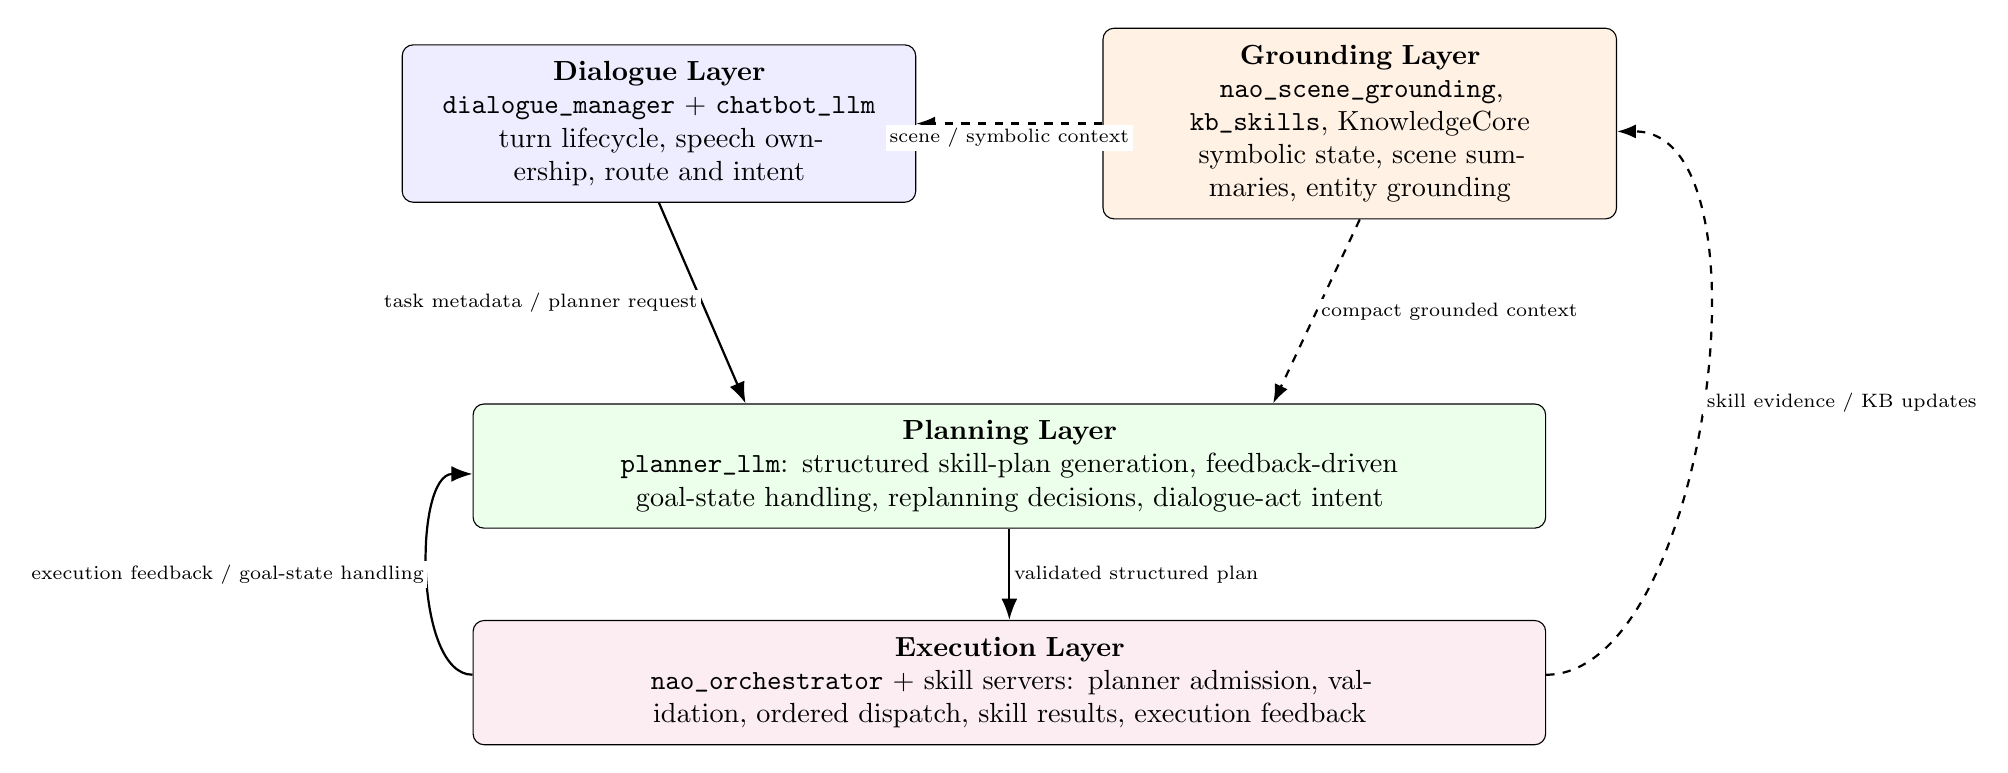
\begin{tikzpicture}[
  font=\normalsize,
  >=Latex,
  box/.style={
    draw,
    rounded corners,
    align=center,
    inner sep=6pt
  },
  topbox/.style={
    box,
    text width=6.1cm,
    minimum height=1.70cm
  },
  widebox/.style={
    box,
    text width=13.2cm,
    minimum height=1.30cm
  },
  control/.style={-{Latex[length=2.7mm]}, thick},
  support/.style={-{Latex[length=2.4mm]}, thick, dashed},
  label/.style={font=\scriptsize, fill=white, inner sep=1.3pt}
]

% Top row: dialogue and grounding are parallel inputs.
\node[topbox, fill=blue!7] (dialogue) at (-4.45,0)
{\textbf{Dialogue Layer}\\
\code{dialogue_manager} + \code{chatbot_llm}\\
turn lifecycle, speech ownership, route and intent};

\node[topbox, fill=orange!10] (grounding) at (4.45,0)
{\textbf{Grounding Layer}\\
\code{nao_scene_grounding}, \code{kb_skills}, KnowledgeCore\\
symbolic state, scene summaries, entity grounding};

% Main layers, with enough vertical spacing to avoid overlap.
\node[widebox, fill=green!8] (planning) at (0,-4.35)
{\textbf{Planning Layer}\\
\code{planner_llm}: structured skill-plan generation, feedback-driven goal-state handling, replanning decisions, dialogue-act intent};

\node[widebox, fill=purple!7] (execution) at (0,-7.10)
{\textbf{Execution Layer}\\
\code{nao_orchestrator} + skill servers: planner admission, validation, ordered dispatch, skill results, execution feedback};

% Grounding also supports chatbot interpretation.
\draw[support]
  (grounding.west) -- node[label, below]{scene / symbolic context}
  (dialogue.east);

% Parallel inputs into the planner.
\draw[control]
  (dialogue.south) -- node[label, left]{task metadata / planner request}
  ([xshift=-3.35cm]planning.north);

\draw[support]
  (grounding.south) -- node[label, right]{compact grounded context}
  ([xshift=3.35cm]planning.north);

% Planner to execution.
\draw[control]
  (planning.south) -- node[label, right]{validated structured plan}
  (execution.north);

% Feedback loop, kept close to avoid shrinking the whole figure.
\draw[control]
  ([yshift=0.10cm]execution.west) to[out=180,in=180,looseness=0.75]
  node[label, left]{execution feedback / goal-state handling}
  ([yshift=-0.10cm]planning.west);

% Evidence update loop, kept close to avoid widening the bounding box.
\draw[support]
  ([yshift=0.10cm]execution.east) to[out=0,in=0,looseness=0.75]
  node[label, right]{skill evidence / KB updates}
  ([yshift=-0.10cm]grounding.east);

\end{tikzpicture}%
}
\caption{High-level layered architecture. Dialogue interpretation and symbolic grounding provide parallel inputs to the planning layer. The chatbot layer also consumes symbolic scene context. The planner proposes structured skill plans, while the execution layer validates and dispatches skills before returning feedback for replanning or dialogue.}
\label{fig:layered-architecture}
\end{figure}

% ============================================================
% Runtime flow
% ============================================================

\subsection{Runtime Flow}

Figure~\ref{fig:runtime-sequence} expands the layered view into the normal execution sequence. The numbered stages distinguish user-turn ownership, planner admission, candidate plan generation, deterministic dispatch, fresh skill evidence, and the return path for replanning or user communication.

\begin{figure}[H]
\centering
\resizebox{0.90\textwidth}{!}{%
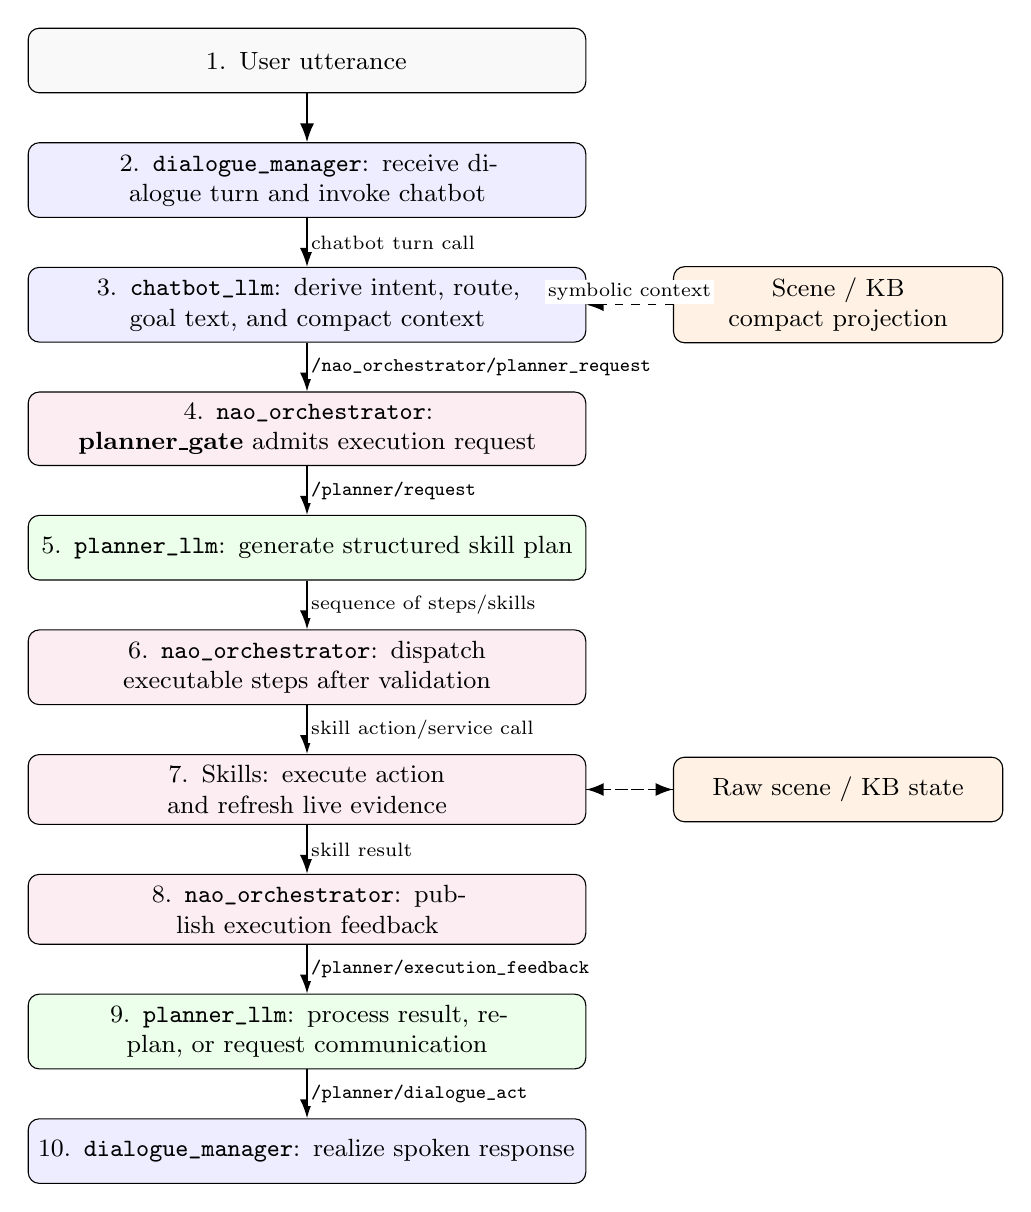
\begin{tikzpicture}[
  font=\small,
  >=Latex,
  node distance=0.58cm,
  box/.style={
    draw,
    rounded corners,
    align=center,
    text width=6.8cm,
    minimum height=0.82cm,
    fill=gray!5,
    inner sep=4pt
  },
  dialogue/.style={box,fill=blue!7},
  planning/.style={box,fill=green!8},
  execution/.style={box,fill=purple!7},
  evidence/.style={
    draw,
    rounded corners,
    align=center,
    text width=3.9cm,
    minimum height=0.82cm,
    fill=orange!10,
    inner sep=4pt
  },
  arr/.style={-{Latex[length=2.4mm]},line width=0.65pt},
  side/.style={-{Latex[length=2.2mm]},line width=0.55pt,dashed},
  edgelabel/.style={font=\scriptsize,fill=white,inner sep=1.2pt}
]

\node[box] (u) {1. User utterance};

\node[dialogue,below=0.62cm of u] (dm)
{2. \code{dialogue_manager}: receive dialogue turn and invoke chatbot};

\node[dialogue,below=0.62cm of dm] (c)
{3. \code{chatbot_llm}: derive intent, route, goal text, and compact context};

\node[execution,below=0.62cm of c] (g)
{4. \code{nao_orchestrator}:\\ \textbf{planner\_gate} admits execution request};

\node[planning,below=0.62cm of g] (p)
{5. \code{planner_llm}: generate structured skill plan};

\node[execution,below=0.62cm of p] (o)
{6. \code{nao_orchestrator}: dispatch executable steps after validation};

\node[execution,below=0.62cm of o] (s)
{7. Skills: execute action and refresh live evidence};

\node[execution,below=0.62cm of s] (f)
{8. \code{nao_orchestrator}: publish execution feedback};

\node[planning,below=0.62cm of f] (sup)
{9. \code{planner_llm}: process result, replan, or request communication};

\node[dialogue,below=0.62cm of sup] (d)
{10. \code{dialogue_manager}: realize spoken response};

\node[evidence,right=1.10cm of c] (kb1)
{Scene / KB\\compact projection};

\node[evidence,right=1.10cm of s] (kb2)
{Raw scene / KB state};

\draw[arr] (u) -- (dm);
\draw[arr] (dm) -- node[edgelabel,right]{chatbot turn call} (c);
\draw[arr] (c) -- node[edgelabel,right]{\code{/nao_orchestrator/planner_request}} (g);
\draw[arr] (g) -- node[edgelabel,right]{\code{/planner/request}} (p);
\draw[arr] (p) -- node[edgelabel,right]{sequence of steps/skills} (o);
\draw[arr] (o) -- node[edgelabel,right]{skill action/service call} (s);
\draw[arr] (s) -- node[edgelabel,right]{skill result} (f);
\draw[arr] (f) -- node[edgelabel,right]{\code{/planner/execution_feedback}} (sup);
\draw[arr] (sup) -- node[edgelabel,right]{\code{/planner/dialogue_act}} (d);

% Grounding/evidence support paths.
\draw[side] (kb1) -- node[edgelabel,above]{symbolic context} (c);
\draw[side] (s) -- (kb2);
\draw[side] (kb2) -- (s);

\end{tikzpicture}%
}
\caption{Runtime message and responsibility sequence from user input to spoken response. The colour coding follows Figure~\ref{fig:layered-architecture}: dialogue components are blue, grounding and evidence are orange, planning is green, and execution is purple.}
\label{fig:runtime-sequence}
\end{figure}

% ============================================================

\section{Runtime Interfaces and Data Contracts}
\label{sec:runtime-contracts}
% ============================================================

The implemented components exchange structured messages so that a language-model output cannot become a robot action without validation. Each contract below identifies the data that crosses one implementation boundary and the component that produces, checks, or consumes it.

\subsection{Runtime Contract Overview}

Table~\ref{tab:contract-map} summarises each runtime contract, its interface or payload, and its owner.

\begin{table}[H]
\centering
\scriptsize
\renewcommand{\arraystretch}{1.18}
\caption{Runtime contract map and ownership in the active dialogue, planning, and execution stack.}
\label{tab:contract-map}

\begin{tabularx}{\textwidth}{
@{}
>{\raggedright\arraybackslash}p{0.04\textwidth}
>{\raggedright\arraybackslash}p{0.17\textwidth}
>{\raggedright\arraybackslash}p{0.38\textwidth}
>{\raggedright\arraybackslash}X
@{}}
\toprule
\textbf{ID} & \textbf{Contract} & \textbf{Interface / payload} & \textbf{Ownership}\\
\midrule

1 & Chatbot turn output
& Internal chatbot result before ROS planner publication.
& \code{dialogue_manager} invokes the chatbot path; \code{chatbot_llm} produces the semantic result.\\

2 & Planner request and admission
& Candidate topic \code{/nao_orchestrator/planner_request}. Admitted topic \code{/planner/request}. Planner-facing payload is carried in \code{Intent.data}.
& \code{chatbot_llm} proposes the execution request; \code{nao_orchestrator} admits and normalizes it; \code{planner_llm} consumes the admitted request.\\

3 & Compact grounding
& \code{grounded_context} inside Contract~2.
& Scene and KB projection provide compact symbolic context for \code{chatbot_llm} and \code{planner_llm}.\\

4 & Shared skill entry
& Registry projection consumed by the planner and orchestrator; its adapter mapping identifies the receiving skill server.
& \code{skill_common} defines the shared capability shape; \code{planner_llm} uses it for prompt construction and \code{nao_orchestrator} uses it for plan validation and dispatch.\\

5 & Planner output
& Topic \code{/intents}. Structured plan payload in \code{Intent.data.plan}.
& \code{planner_llm} produces the plan; \code{nao_orchestrator} validates and dispatches executable steps.\\

6 & Skill execution result
& ROS action result or service response with a typed skill-result payload.
& \code{nao_orchestrator} dispatches the call; the skill server owns fresh evidence; verified world-state updates are applied through \code{kb_skills}.\\

7 & Execution feedback
& Topic \code{/planner/execution_feedback}. Structured JSON feedback payload.
& \code{nao_orchestrator} publishes feedback; a goal-keyed planning-state helper inside \code{planner_llm} uses it for replanning, clarification, or failure handling.\\

8 & Planner dialogue act
& Topic \code{/planner/dialogue_act}. Structured communication request.
& \code{planner_llm} emits dialogue-act intent; \code{nao_orchestrator} relays it; \code{dialogue_manager} realizes the final speech.\\

9 & RDF knowledge state and raw evidence
& KnowledgeCore statements through \code{/kb/query} and \code{/kb/revise}; source evidence includes tracked-person state, \code{/scene/summary}, and skill results.
& Source components own fact freshness; \code{kb_skills} owns KB transport; compact projections and feedback preserve provenance without replacing raw evidence.\\

\bottomrule
\end{tabularx}
\end{table}

The overview keeps only the fields needed to identify each contract. Later sections add the runtime metadata needed for orchestration, feedback-driven planning, tracing, and debugging.

\subsection{Contract 1: Chatbot Turn Output}

The intent in this contract is the user's goal as extracted by the chatbot. It is not a planner output.

\begin{lstlisting}
{
  "verbal_ack": "Okay, I will do that.",
  "route": "execution",
  "confidence": 0.82,
  "user_intent": {
    "type": "look_at",
    "goal_text": "look at the person",
    "scene_targets": ["person"],
    "request_kind": "new_goal"
  }
}
\end{lstlisting}

Table~\ref{tab:chatbot-fields} identifies the fields that remain visible after the chatbot completes one semantic routing decision.

\begin{table}[H]
\centering
\footnotesize
\renewcommand{\arraystretch}{1.18}
\caption{Fields in Contract 1: chatbot turn output.}
\label{tab:chatbot-fields}

\begin{tabularx}{\textwidth}{
@{}
>{\raggedright\arraybackslash}p{0.33\textwidth}
>{\raggedright\arraybackslash}X
@{}}
\toprule
\textbf{Field} & \textbf{Meaning}\\
\midrule

\code{verbal_ack}
& Optional immediate acknowledgement generated by the chatbot layer. This may be spoken or logged before execution begins, depending on the dialogue policy.\\

\code{route}
& Turn classification produced by \code{chatbot_llm}. Supported values include \code{dialogue}, \code{knowledge_query}, and \code{execution}. Only \code{execution} turns enter the planner path; \code{dialogue} and \code{knowledge_query} remain non-execution turns but are still useful for tracing.\\

\code{confidence}
& Confidence assigned by the chatbot or intent-extraction stage. It is useful for debugging and possible admission policy, but it is not a planner priority score.\\

\code{user_intent.type}
& Normalized user-intent label extracted by \code{chatbot_llm}, such as \code{look_at}, \code{find_object}, \code{scan}, or \code{navigate_to}.\\

\code{user_intent.goal_text}
& Natural-language objective passed toward the planner path as the task to satisfy. This field preserves the user's goal in a compact form.\\

\begin{tabular}[t]{@{}l@{}}
\code{user_intent.}\\
\code{scene_targets}
\end{tabular}
& Optional target hints extracted from the utterance, such as \code{person}, \code{cup}, or \code{table}. These are hints, not validated grounded entities.\\

\begin{tabular}[t]{@{}l@{}}
\code{user_intent.}\\
\code{request_kind}
\end{tabular}
& Proposed goal transition class, such as \code{new_goal}, \code{update_goal}, \code{answer_to_clarification}, or \code{cancel_goal}. The planner gate inside \code{nao_orchestrator} should normalize and admit this field before publishing \code{/planner/request}.\\

\bottomrule
\end{tabularx}
\end{table}


\subsection{Contract 2: Planner Request}

The planner request is the task description generated by the orchestrator from the chatbot output and consumed by the planner.

\begin{lstlisting}
{
  "goal_id": "goal_turn_123",
  "request_kind": "new_goal",
  "goal_text": "look at the person and report completion",
  "normalized_intents": ["look_at"],
  "grounded_context": {
    "entities": [
      {
        "id": "anonymous_person_ehfbf",
        "label": null,
        "kind": "person",
        "class": "Human",
        "visible": true,
        "relations": []
      }
    ]
  }
}
\end{lstlisting}

Table~\ref{tab:planner-request-fields} separates request identity, goal semantics, and grounded evidence before the planner is invoked.

\begin{table}[H]
\centering
\footnotesize
\renewcommand{\arraystretch}{1.18}
\caption{Fields in Contract 2: minimal planner-facing request.}
\label{tab:planner-request-fields}

\begin{tabularx}{\textwidth}{
@{}
>{\raggedright\arraybackslash}p{0.33\textwidth}
>{\raggedright\arraybackslash}X
@{}}
\toprule
\textbf{Field} & \textbf{Meaning}\\
\midrule

\code{goal_id}
& Identifier for the active objective. It groups replans and feedback for the same task.\\

\code{request_kind}
& States whether this is a new goal, an update to the current goal, a cancellation, or another supported transition. \code{chatbot_llm} may propose it, but \code{nao_orchestrator} normalizes and admits it before publishing \code{/planner/request}.\\

\code{goal_text}
& Objective extracted from the user utterance. This is the central planning input for \code{planner_llm}.\\

\code{normalized_intents}
& Intent labels extracted by \code{chatbot_llm}. They help \code{planner_llm} choose suitable skills from the available skill registry.\\

\code{grounded_context}
& Compact scene graph used by the planner as the current symbolic state of the world. It contains validated entities and relations rather than raw detector output.\\

\bottomrule
\end{tabularx}
\end{table}

\subsection{Contract 3: Grounded Context}

The planner receives a compact, JSON-native view of relevant world state. This is best described as a compact scene graph derived from the KB, continually updated by the perception pipeline (human/person detection and object perception). Raw KB triples, detector metadata, and tracker-derived details remain available through scene/KB evidence paths to skills, but they are not duplicated into every LLM prompt.

\Needspace{18\baselineskip}
\begin{lstlisting}
{
  "grounded_context": {
    "entities": [
      {
        "id": "cup_jrjic",
        "label": "cup",
        "kind": "object",
        "class": "Cup",
        "visible": true,
        "relations": [
          {"predicate": "dbp:color", "object": "blue"},
          {"predicate": "oro:isOn", "object": "table_1"}
        ]
      },
      {
        "id": "anonymous_person_ehfbf",
        "label": null,
        "kind": "person",
        "class": "Human",
        "visible": true,
        "relations": []
      }
    ]
  }
}
\end{lstlisting}

Table~\ref{tab:grounded-context-fields} defines the compact entity and relation fields used by dialogue and planning.

\begin{table}[H]
\centering
\footnotesize
\renewcommand{\arraystretch}{1.18}
\caption{Fields in Contract 3: grounded context.}
\label{tab:grounded-context-fields}

\begin{tabularx}{\textwidth}{
@{}
>{\raggedright\arraybackslash}p{0.33\textwidth}
>{\raggedright\arraybackslash}X
@{}}
\toprule
\textbf{Field} & \textbf{Meaning}\\
\midrule

\code{id}
& Stable entity handle used by planner steps and skill arguments. This is the preferred reference when a skill needs to target a known person, object, or location.\\

\code{label}
& Human-readable name or class hint. It may be empty for anonymous people or entities that should not be assigned a personal name.\\

\code{kind}
& Entity category, such as \code{object}, \code{person}, or another supported runtime category. This prevents people from being treated as generic objects.\\

\code{class}
& Compact semantic class used by the planner for reasoning, such as \code{Cup}, \code{Human}, or \code{Table}.\\

\code{visible}
& Indicates whether the entity is currently grounded in the latest accepted scene or KB state. It should not be treated as a guarantee that the entity will still be available at execution time.\\

\code{relations}
& Bounded list of relevant semantic relations, such as colour, containment, support, proximity, or ownership-style facts. These relations add task-relevant context without exposing the full KB.\\

\bottomrule
\end{tabularx}
\end{table}

\subsection{Contract 4: Shared Skill Entry}

The planner and orchestrator use one shared entry shape to describe a skill before it is placed in a prompt, admitted for execution, or mapped to an action server. The entry separates the information needed to select a skill from the information needed to verify its result.

\begin{lstlisting}
{
  "object_id": "navigate_to",
  "kind": "skill",
  "category": "navigation",
  "aliases": ["go_to", "move_to_location"],
  "params": ["target", "location"],
  "required_params": ["target"],
  "preconditions": ["navigation is enabled",
                    "target is known or resolvable"],
  "expected_effects": ["robot arrives at the target location"],
  "observable_success": ["status"],
  "failure_modes": ["path_blocked", "unknown_location",
                    "safety_disabled"],
  "planner_guidance": ["use for a semantic destination"],
  "result_schema": {"required": ["skill", "status", "summary_text"]},
  "safety_flags": ["navigation"],
  "implementation_status": "fake",
  "robot_adapter_mapping": "fake_skills.navigate_to",
  "supports_failure_injection": true,
  "metadata": {"runtime_callable": true}
}
\end{lstlisting}

Table~\ref{tab:skill-entry-contract} names the common capability fields consumed by prompt construction, admission, dispatch, and result interpretation.

\begin{table}[H]
\centering
\footnotesize
\renewcommand{\arraystretch}{1.15}
\caption{Shared skill-entry fields used by planning and execution.}
\label{tab:skill-entry-contract}
\begin{tabularx}{\textwidth}{
@{}
>{\raggedright\arraybackslash}p{0.25\textwidth}
>{\raggedright\arraybackslash}X
@{}}
\toprule
\textbf{Field} & \textbf{Runtime role}\\
\midrule
\code{object_id}, \code{kind}, \code{category}, \code{aliases}
& Canonical planner name, semantic group, and accepted compatibility names.\\
\code{params}, \code{required_params}
& Typed planner-facing arguments and the subset required before admission.\\
\code{preconditions}
& Grounding or state assumptions that must be satisfied or explicitly owned by a scenario. They do not prove a future effect.\\
\code{expected_effects}
& Intended state changes or evidence products used to select and order skills.\\
\code{observable_success}
& Result or trace evidence that can support completion after execution.\\
\code{failure_modes}
& Typed outcomes used by the orchestrator and the goal-state helper to stop, clarify, or request replanning.\\
\code{planner_guidance}
& Bounded selection and ordering guidance inserted into the planner prompt.\\
\code{result_schema}
& Required and optional result fields, including the summary and evidence payload.\\
\code{safety_flags}
& Safety-relevant labels used during admission and dispatch.\\
\path{metadata.runtime_callable}
& Whether the registry permits planner-visible runtime use.\\
\code{implementation_status}
& Current implementation class, such as first-party, fake, or hybrid.\\
\code{robot_adapter_mapping}
& Adapter or skill server that receives the dispatched call.\\
\code{supports_failure_}\newline\code{injection}
& Whether controlled failure outcomes are available for validation.\\
\bottomrule
\end{tabularx}
\end{table}

The same shape is projected to the planner prompt, deterministic orchestrator checks, controlled fake skill simulation policies, and adapter configuration. Preconditions constrain admission, while expected effects remain hypotheses until a skill returns observable evidence. This distinction is used by \code{report_result}: a final summary must be derived from result payloads or trace evidence rather than copied from a planner-generated claim. The complete runtime inventory is provided in Appendix~\ref{sec:runtime-skill-inventory}.

\subsection{Contract 5: Planner Output}

The planner output is a plan: a sequence of skill steps to achieve the user goal. It should focus on executable content and minimal lineage. Communication policy and retry metadata are still valid runtime fields when used by the stack, but this controlled version foregrounds the ordered \code{steps} list because that is the essential planner output.

\Needspace{18\baselineskip}
\begin{lstlisting}
{
  "plan": {
    "goal_id": "goal_turn_123",
    "plan_id": "plan_123",
    "plan_version": 1,
    "status": "planned",
    "steps": [
      {
        "id": "step_1",
        "type": "skill",
        "name": "look_at",
        "args": {"target_frame": "anonymous_person_ehfbf"},
        "requires": [],
        "on_failure": "replan"
      }
    ]
  }
}
\end{lstlisting}

Table~\ref{tab:planner-output-fields} identifies the plan and step fields that must survive deterministic validation before dispatch.

\begin{table}[H]
\centering
\footnotesize
\renewcommand{\arraystretch}{1.18}
\caption{Fields in Contract 5: planner output.}
\label{tab:planner-output-fields}

\begin{tabularx}{\textwidth}{
@{}
>{\raggedright\arraybackslash}p{0.32\textwidth}
>{\raggedright\arraybackslash}X
@{}}
\toprule
\textbf{Field} & \textbf{Meaning}\\
\midrule

\code{goal_id}
& User objective that this plan attempts to satisfy. It links the planner output to the active goal.\\

\code{plan_id}
& Identifier for this concrete plan proposal. It is useful when the runtime keeps plan history or compares revised plans for the same goal.\\

\code{plan_version}
& Revision number for replans of the same goal. This helps distinguish the initial plan from later feedback-driven planning outputs.\\

\code{status}
& Planning outcome for this plan, such as \code{planned}, \code{needs_clarification}, or \code{failed_to_plan}. This describes whether \code{planner_llm} produced an executable plan, not whether the robot has already executed it.\\

\code{steps}
& Ordered list of skill calls produced by the planner. This is the essential planner output consumed by \code{nao_orchestrator}.\\

\code{steps[].id}
& Stable step identifier used for execution feedback, dependency tracking, and possible replan joins.\\

\code{steps[].name}
& Skill name selected from the allowed skill registry. The planner should not invent skills or use robot-specific APIs directly.\\

\code{steps[].args}
& Skill arguments. They should refer to known entity IDs, explicit primitive values, or arguments supported by the selected skill schema.\\

\code{steps[].requires}
& Dependencies between steps, if any. This allows the runtime to know which steps depend on previous successful outcomes.\\

\begin{tabular}[t]{@{}l@{}}
\code{steps[].}\\
\code{on_failure}
\end{tabular}
& Recovery policy proposed by \code{planner_llm} for this step. If the step fails, \code{nao_orchestrator} may fail safely, continue if allowed, request user input, or send feedback back to \code{planner_llm} for replanning. Allowed values include \code{replan}, \code{clarify}, \code{ask_user}, \code{continue}, \code{ignore}, and \code{fail}.\\

\bottomrule
\end{tabularx}
\end{table}

\paragraph{Runtime recovery metadata.}
The current contract supports recovery metadata as skill failure may require controlled recovery. Each step may carry a \code{retry_budget}, and the plan envelope may also carry a plan-level \code{retry_budget}. This does not mean that \code{retry} is a separate \code{on_failure} value. Instead, retry behaviour is controlled by \code{nao_orchestrator} using the available retry budget together with the step's \code{on_failure} policy. The plan envelope may also carry \code{communication_policy}. This controls when the planner/dialogue path should communicate progress, completion, clarification needs, or failure.

When a step fails with \code{on_failure = replan}, \code{nao_orchestrator} halts or blocks continuation, publishes execution feedback to \code{planner_llm}, and waits for a revised validated plan before dispatching further actions. This keeps execution authority inside \code{nao_orchestrator}, while allowing recovery to be driven by feedback-driven planning rather than by hard-coded local replanning.

\subsection{Contract 6: Skill Execution Result}

Every dispatched skill returns a typed result before the orchestrator can mark its step as completed. The result distinguishes the execution status from the evidence that supports it. For state-changing skills, the evidence may also describe world-state changes that must be reflected in the KB. These changes are reported by the skill that observed or produced them; they are not inferred from the planner's expected-effects text in Contract~4.

\begin{lstlisting}
{
  "skill": "place_object",
  "status": "succeeded",
  "summary_text": "I placed cup_1 on table_1.",
  "evidence": {
    "object_id": "cup_1",
    "destination_id": "table_1",
    "kb_effects": [
      {"operation": "remove", "statement": "robot oro:holds cup_1"},
      {"operation": "add", "statement": "cup_1 oro:isOn table_1"}
    ]
  },
  "failure": null,
  "metadata": {"fake": true}
}
\end{lstlisting}

The implementation retains the field name \code{evidence.kb_effects}, but the field describes observed world-state changes that must be reflected in the KB and the orchestrator applies these statements only after a successful result.

\subsection{Contract 7: Execution Feedback}

Execution feedback tells the planner which goal and step were affected, whether the step succeeded or failed, and why. This compact information is sufficient to decide whether to continue, replan, request clarification, or report failure.

\Needspace{18\baselineskip}
\begin{lstlisting}
{
  "goal_id": "goal_turn_123",
  "status": "failed",
  "step": {
    "id": "step_1",
    "name": "look_at"
  },
  "reason": "target frame unavailable",
  "result_payload": {
    "target_found": false,
    "target_kind": "person"
  }
}
\end{lstlisting}



Runtime feedback may include additional fields used by \code{nao_orchestrator}, logging, and the goal-state helper. Lineage uses \code{plan_id} and \code{plan_version}; event handling may add \code{event_type}, \code{validation_status}, \code{blocking}, and \path{needs_user_input}; observability may add \code{timestamp_sec}, \code{result_summary}, and retry metadata. These fields support execution control and debugging, while the minimal planner-facing feedback remains the goal, step, status, reason, and result payload.

\subsection{Contract 8: Planner Dialogue Act}

Planner dialogue acts represent planner intent to communicate, not direct speech execution. They are relayed through the orchestrator and realized by the dialogue layer.

\begin{lstlisting}
{
  "goal_id": "goal_turn_123",
  "act": "ask_clarification",
  "await_user_response": true,
  "reason": "multiple visible people",
  "text_hint": "Which person should I look at?",
  "slots_needed": ["target_person"]
}
\end{lstlisting}

Allowed dialogue acts are acknowledgement, progress update, clarification, help request, failure explanation, completion notification, and cancellation notification. The planner does not speak directly; it emits a structured communication request.

\subsection{Contract 9: RDF Knowledge State}

The implementation reuses the open-source KnowledgeCore package rather than introducing a new knowledge-base system \parencite{knowledgecore}. KnowledgeCore represents symbolic world state as an RDF-style graph. Each statement has a subject, predicate, and object. Stable subjects identify people, objects, places, supports, and the robot; predicates express class membership, attributes, visibility, containment, and spatial relations. The same statement shape is used by preloaded fixtures, detector-derived object facts, explicit user-authorised KB mutations, and verified post-skill effects.

\begin{lstlisting}
codex_lab_cup rdf:type Cup
codex_lab_cup dbp:color red
codex_lab_cup oro:isOn codex_lab_table
codex_lab_room oro:contains codex_lab_table
person_alex rdf:type Human
myself sees person_alex
\end{lstlisting}

The principal predicate families are shown in Table~\ref{tab:rdf-kb-predicates}. A class statement such as \code{rdf:type Human} also preserves the semantic distinction between a person and an object even when both can be action targets.

\begin{table}[H]
\centering
\footnotesize
\renewcommand{\arraystretch}{1.15}
\caption{Principal RDF-style predicate families used by the runtime KB.}
\label{tab:rdf-kb-predicates}
\begin{tabularx}{\textwidth}{@{}p{0.24\textwidth}p{0.29\textwidth}X@{}}
\toprule
\textbf{Role} & \textbf{Representative predicates} & \textbf{Runtime meaning}\\
\midrule
Entity class & \code{rdf:type} & Distinguishes people, objects, supports, rooms, and other planner-relevant classes.\\
Attributes & \code{dbp:name}, \code{dbp:color} & Provides stable semantic labels and disambiguating properties.\\
Observation & \code{sees}, visual-centre, score, source, and last-seen predicates & Records who observed an entity and the bounded provenance/freshness of a detector observation.\\
Spatial relations & \code{oro:isOn}, \code{oro:isAt}, \code{oro:isIn}, \code{oro:contains} & Represents support, destination, room membership, and containment used by grounding and skill effects.\\
\bottomrule
\end{tabularx}
\end{table}

KB mutations use add, revise, and remove operations on this shared statement form through \code{/kb/revise}; reads use query patterns through \code{/kb/query}. Transient perception facts carry a finite lifespan, while explicit fixture and verified skill-effect facts follow the lifetime declared by their owner. Reused person-perception components publish person identities and tracked state through their public interfaces \parencite{mohamed2020ros4hri}. Object detections are handled separately by \code{nao_scene_grounding}, which publishes \code{/scene/summary} and detector-derived KB statements.

% ============================================================

\chapter{Implementation}
\label{chap:implementation}
\label{sec:implementation}

This chapter describes how the architecture introduced in Chapter~\ref{chap:architecture-requirements} is realised in the ROS~2 workspace. The implementation separates semantic interpretation, planning, deterministic execution, perception grounding, symbolic knowledge, and robot skills. Language-model components interpret requests and propose actions, while typed ROS~2 interfaces and the orchestrator govern execution.

The workspace combines locally developed integration packages with reusable HRI and knowledge components. The implemented contribution is the integration of dialogue management, semantic routing, grounding, planning, orchestration, skills, and feedback into a coherent runtime for the NAO platform.

\section{Runtime Interfaces and Data Contracts}
\label{sec:runtime-contracts}
% ============================================================

The implemented components exchange structured messages so that a language-model output cannot become a robot action without validation. Each contract below identifies the data that crosses one implementation boundary and the component that produces, checks, or consumes it.

\subsection{Runtime Contract Overview}

Table~\ref{tab:contract-map} summarises each runtime contract, its interface or payload, and its owner.

\begin{table}[H]
\centering
\scriptsize
\renewcommand{\arraystretch}{1.18}
\caption{Runtime contract map and ownership in the active dialogue, planning, and execution stack.}
\label{tab:contract-map}

\begin{tabularx}{\textwidth}{
@{}
>{\raggedright\arraybackslash}p{0.04\textwidth}
>{\raggedright\arraybackslash}p{0.17\textwidth}
>{\raggedright\arraybackslash}p{0.38\textwidth}
>{\raggedright\arraybackslash}X
@{}}
\toprule
\textbf{ID} & \textbf{Contract} & \textbf{Interface / payload} & \textbf{Ownership}\\
\midrule

1 & Chatbot turn output
& Internal chatbot result before ROS planner publication.
& \code{dialogue_manager} invokes the chatbot path; \code{chatbot_llm} produces the semantic result.\\

2 & Planner request and admission
& Candidate topic \code{/nao_orchestrator/planner_request}. Admitted topic \code{/planner/request}. Planner-facing payload is carried in \code{Intent.data}.
& \code{chatbot_llm} proposes the execution request; \code{nao_orchestrator} admits and normalizes it; \code{planner_llm} consumes the admitted request.\\

3 & Compact grounding
& \code{grounded_context} inside Contract~2.
& Scene and KB projection provide compact symbolic context for \code{chatbot_llm} and \code{planner_llm}.\\

4 & Shared skill entry
& Registry projection consumed by the planner and orchestrator; its adapter mapping identifies the receiving skill server.
& \code{skill_common} defines the shared capability shape; \code{planner_llm} uses it for prompt construction and \code{nao_orchestrator} uses it for plan validation and dispatch.\\

5 & Planner output
& Topic \code{/intents}. Structured plan payload in \code{Intent.data.plan}.
& \code{planner_llm} produces the plan; \code{nao_orchestrator} validates and dispatches executable steps.\\

6 & Skill execution result
& ROS action result or service response with a typed skill-result payload.
& \code{nao_orchestrator} dispatches the call; the skill server owns fresh evidence; verified world-state updates are applied through \code{kb_skills}.\\

7 & Execution feedback
& Topic \code{/planner/execution_feedback}. Structured JSON feedback payload.
& \code{nao_orchestrator} publishes feedback; a goal-keyed planning-state helper inside \code{planner_llm} uses it for replanning, clarification, or failure handling.\\

8 & Planner dialogue act
& Topic \code{/planner/dialogue_act}. Structured communication request.
& \code{planner_llm} emits dialogue-act intent; \code{nao_orchestrator} relays it; \code{dialogue_manager} realizes the final speech.\\

9 & RDF knowledge state and raw evidence
& KnowledgeCore statements through \code{/kb/query} and \code{/kb/revise}; source evidence includes tracked-person state, \code{/scene/summary}, and skill results.
& Source components own fact freshness; \code{kb_skills} owns KB transport; compact projections and feedback preserve provenance without replacing raw evidence.\\

\bottomrule
\end{tabularx}
\end{table}

The overview keeps only the fields needed to identify each contract. Later sections add the runtime metadata needed for orchestration, feedback-driven planning, tracing, and debugging.

\subsection{Contract 1: Chatbot Turn Output}

The intent in this contract is the user's goal as extracted by the chatbot. It is not a planner output.

\begin{lstlisting}
{
  "verbal_ack": "Okay, I will do that.",
  "route": "execution",
  "confidence": 0.82,
  "user_intent": {
    "type": "look_at",
    "goal_text": "look at the person",
    "scene_targets": ["person"],
    "request_kind": "new_goal"
  }
}
\end{lstlisting}

Table~\ref{tab:chatbot-fields} identifies the fields that remain visible after the chatbot completes one semantic routing decision.

\begin{table}[H]
\centering
\footnotesize
\renewcommand{\arraystretch}{1.18}
\caption{Fields in Contract 1: chatbot turn output.}
\label{tab:chatbot-fields}

\begin{tabularx}{\textwidth}{
@{}
>{\raggedright\arraybackslash}p{0.33\textwidth}
>{\raggedright\arraybackslash}X
@{}}
\toprule
\textbf{Field} & \textbf{Meaning}\\
\midrule

\code{verbal_ack}
& Optional immediate acknowledgement generated by the chatbot layer. This may be spoken or logged before execution begins, depending on the dialogue policy.\\

\code{route}
& Turn classification produced by \code{chatbot_llm}. Supported values include \code{dialogue}, \code{knowledge_query}, and \code{execution}. Only \code{execution} turns enter the planner path; \code{dialogue} and \code{knowledge_query} remain non-execution turns but are still useful for tracing.\\

\code{confidence}
& Confidence assigned by the chatbot or intent-extraction stage. It is useful for debugging and possible admission policy, but it is not a planner priority score.\\

\code{user_intent.type}
& Normalized user-intent label extracted by \code{chatbot_llm}, such as \code{look_at}, \code{find_object}, \code{scan}, or \code{navigate_to}.\\

\code{user_intent.goal_text}
& Natural-language objective passed toward the planner path as the task to satisfy. This field preserves the user's goal in a compact form.\\

\begin{tabular}[t]{@{}l@{}}
\code{user_intent.}\\
\code{scene_targets}
\end{tabular}
& Optional target hints extracted from the utterance, such as \code{person}, \code{cup}, or \code{table}. These are hints, not validated grounded entities.\\

\begin{tabular}[t]{@{}l@{}}
\code{user_intent.}\\
\code{request_kind}
\end{tabular}
& Proposed goal transition class, such as \code{new_goal}, \code{update_goal}, \code{answer_to_clarification}, or \code{cancel_goal}. The planner gate inside \code{nao_orchestrator} should normalize and admit this field before publishing \code{/planner/request}.\\

\bottomrule
\end{tabularx}
\end{table}


\subsection{Contract 2: Planner Request}

The planner request is the task description generated by the orchestrator from the chatbot output and consumed by the planner.

\begin{lstlisting}
{
  "goal_id": "goal_turn_123",
  "request_kind": "new_goal",
  "goal_text": "look at the person and report completion",
  "normalized_intents": ["look_at"],
  "grounded_context": {
    "entities": [
      {
        "id": "anonymous_person_ehfbf",
        "label": null,
        "kind": "person",
        "class": "Human",
        "visible": true,
        "relations": []
      }
    ]
  }
}
\end{lstlisting}

Table~\ref{tab:planner-request-fields} separates request identity, goal semantics, and grounded evidence before the planner is invoked.

\begin{table}[H]
\centering
\footnotesize
\renewcommand{\arraystretch}{1.18}
\caption{Fields in Contract 2: minimal planner-facing request.}
\label{tab:planner-request-fields}

\begin{tabularx}{\textwidth}{
@{}
>{\raggedright\arraybackslash}p{0.33\textwidth}
>{\raggedright\arraybackslash}X
@{}}
\toprule
\textbf{Field} & \textbf{Meaning}\\
\midrule

\code{goal_id}
& Identifier for the active objective. It groups replans and feedback for the same task.\\

\code{request_kind}
& States whether this is a new goal, an update to the current goal, a cancellation, or another supported transition. \code{chatbot_llm} may propose it, but \code{nao_orchestrator} normalizes and admits it before publishing \code{/planner/request}.\\

\code{goal_text}
& Objective extracted from the user utterance. This is the central planning input for \code{planner_llm}.\\

\code{normalized_intents}
& Intent labels extracted by \code{chatbot_llm}. They help \code{planner_llm} choose suitable skills from the available skill registry.\\

\code{grounded_context}
& Compact scene graph used by the planner as the current symbolic state of the world. It contains validated entities and relations rather than raw detector output.\\

\bottomrule
\end{tabularx}
\end{table}

\subsection{Contract 3: Grounded Context}

The planner receives a compact, JSON-native view of relevant world state. This is best described as a compact scene graph derived from the KB, continually updated by the perception pipeline (human/person detection and object perception). Raw KB triples, detector metadata, and tracker-derived details remain available through scene/KB evidence paths to skills, but they are not duplicated into every LLM prompt.

\Needspace{18\baselineskip}
\begin{lstlisting}
{
  "grounded_context": {
    "entities": [
      {
        "id": "cup_jrjic",
        "label": "cup",
        "kind": "object",
        "class": "Cup",
        "visible": true,
        "relations": [
          {"predicate": "dbp:color", "object": "blue"},
          {"predicate": "oro:isOn", "object": "table_1"}
        ]
      },
      {
        "id": "anonymous_person_ehfbf",
        "label": null,
        "kind": "person",
        "class": "Human",
        "visible": true,
        "relations": []
      }
    ]
  }
}
\end{lstlisting}

Table~\ref{tab:grounded-context-fields} defines the compact entity and relation fields used by dialogue and planning.

\begin{table}[H]
\centering
\footnotesize
\renewcommand{\arraystretch}{1.18}
\caption{Fields in Contract 3: grounded context.}
\label{tab:grounded-context-fields}

\begin{tabularx}{\textwidth}{
@{}
>{\raggedright\arraybackslash}p{0.33\textwidth}
>{\raggedright\arraybackslash}X
@{}}
\toprule
\textbf{Field} & \textbf{Meaning}\\
\midrule

\code{id}
& Stable entity handle used by planner steps and skill arguments. This is the preferred reference when a skill needs to target a known person, object, or location.\\

\code{label}
& Human-readable name or class hint. It may be empty for anonymous people or entities that should not be assigned a personal name.\\

\code{kind}
& Entity category, such as \code{object}, \code{person}, or another supported runtime category. This prevents people from being treated as generic objects.\\

\code{class}
& Compact semantic class used by the planner for reasoning, such as \code{Cup}, \code{Human}, or \code{Table}.\\

\code{visible}
& Indicates whether the entity is currently grounded in the latest accepted scene or KB state. It should not be treated as a guarantee that the entity will still be available at execution time.\\

\code{relations}
& Bounded list of relevant semantic relations, such as colour, containment, support, proximity, or ownership-style facts. These relations add task-relevant context without exposing the full KB.\\

\bottomrule
\end{tabularx}
\end{table}

\subsection{Contract 4: Shared Skill Entry}

The planner and orchestrator use one shared entry shape to describe a skill before it is placed in a prompt, admitted for execution, or mapped to an action server. The entry separates the information needed to select a skill from the information needed to verify its result.

\begin{lstlisting}
{
  "object_id": "navigate_to",
  "kind": "skill",
  "category": "navigation",
  "aliases": ["go_to", "move_to_location"],
  "params": ["target", "location"],
  "required_params": ["target"],
  "preconditions": ["navigation is enabled",
                    "target is known or resolvable"],
  "expected_effects": ["robot arrives at the target location"],
  "observable_success": ["status"],
  "failure_modes": ["path_blocked", "unknown_location",
                    "safety_disabled"],
  "planner_guidance": ["use for a semantic destination"],
  "result_schema": {"required": ["skill", "status", "summary_text"]},
  "safety_flags": ["navigation"],
  "implementation_status": "fake",
  "robot_adapter_mapping": "fake_skills.navigate_to",
  "supports_failure_injection": true,
  "metadata": {"runtime_callable": true}
}
\end{lstlisting}

Table~\ref{tab:skill-entry-contract} names the common capability fields consumed by prompt construction, admission, dispatch, and result interpretation.

\begin{table}[H]
\centering
\footnotesize
\renewcommand{\arraystretch}{1.15}
\caption{Shared skill-entry fields used by planning and execution.}
\label{tab:skill-entry-contract}
\begin{tabularx}{\textwidth}{
@{}
>{\raggedright\arraybackslash}p{0.25\textwidth}
>{\raggedright\arraybackslash}X
@{}}
\toprule
\textbf{Field} & \textbf{Runtime role}\\
\midrule
\code{object_id}, \code{kind}, \code{category}, \code{aliases}
& Canonical planner name, semantic group, and accepted compatibility names.\\
\code{params}, \code{required_params}
& Typed planner-facing arguments and the subset required before admission.\\
\code{preconditions}
& Grounding or state assumptions that must be satisfied or explicitly owned by a scenario. They do not prove a future effect.\\
\code{expected_effects}
& Intended state changes or evidence products used to select and order skills.\\
\code{observable_success}
& Result or trace evidence that can support completion after execution.\\
\code{failure_modes}
& Typed outcomes used by the orchestrator and the goal-state helper to stop, clarify, or request replanning.\\
\code{planner_guidance}
& Bounded selection and ordering guidance inserted into the planner prompt.\\
\code{result_schema}
& Required and optional result fields, including the summary and evidence payload.\\
\code{safety_flags}
& Safety-relevant labels used during admission and dispatch.\\
\path{metadata.runtime_callable}
& Whether the registry permits planner-visible runtime use.\\
\code{implementation_status}
& Current implementation class, such as first-party, fake, or hybrid.\\
\code{robot_adapter_mapping}
& Adapter or skill server that receives the dispatched call.\\
\code{supports_failure_}\newline\code{injection}
& Whether controlled failure outcomes are available for validation.\\
\bottomrule
\end{tabularx}
\end{table}

The same shape is projected to the planner prompt, deterministic orchestrator checks, controlled fake skill simulation policies, and adapter configuration. Preconditions constrain admission, while expected effects remain hypotheses until a skill returns observable evidence. This distinction is used by \code{report_result}: a final summary must be derived from result payloads or trace evidence rather than copied from a planner-generated claim. The complete runtime inventory is provided in Appendix~\ref{sec:runtime-skill-inventory}.

\subsection{Contract 5: Planner Output}

The planner output is a plan: a sequence of skill steps to achieve the user goal. It should focus on executable content and minimal lineage. Communication policy and retry metadata are still valid runtime fields when used by the stack, but this controlled version foregrounds the ordered \code{steps} list because that is the essential planner output.

\Needspace{18\baselineskip}
\begin{lstlisting}
{
  "plan": {
    "goal_id": "goal_turn_123",
    "plan_id": "plan_123",
    "plan_version": 1,
    "status": "planned",
    "steps": [
      {
        "id": "step_1",
        "type": "skill",
        "name": "look_at",
        "args": {"target_frame": "anonymous_person_ehfbf"},
        "requires": [],
        "on_failure": "replan"
      }
    ]
  }
}
\end{lstlisting}

Table~\ref{tab:planner-output-fields} identifies the plan and step fields that must survive deterministic validation before dispatch.

\begin{table}[H]
\centering
\footnotesize
\renewcommand{\arraystretch}{1.18}
\caption{Fields in Contract 5: planner output.}
\label{tab:planner-output-fields}

\begin{tabularx}{\textwidth}{
@{}
>{\raggedright\arraybackslash}p{0.32\textwidth}
>{\raggedright\arraybackslash}X
@{}}
\toprule
\textbf{Field} & \textbf{Meaning}\\
\midrule

\code{goal_id}
& User objective that this plan attempts to satisfy. It links the planner output to the active goal.\\

\code{plan_id}
& Identifier for this concrete plan proposal. It is useful when the runtime keeps plan history or compares revised plans for the same goal.\\

\code{plan_version}
& Revision number for replans of the same goal. This helps distinguish the initial plan from later feedback-driven planning outputs.\\

\code{status}
& Planning outcome for this plan, such as \code{planned}, \code{needs_clarification}, or \code{failed_to_plan}. This describes whether \code{planner_llm} produced an executable plan, not whether the robot has already executed it.\\

\code{steps}
& Ordered list of skill calls produced by the planner. This is the essential planner output consumed by \code{nao_orchestrator}.\\

\code{steps[].id}
& Stable step identifier used for execution feedback, dependency tracking, and possible replan joins.\\

\code{steps[].name}
& Skill name selected from the allowed skill registry. The planner should not invent skills or use robot-specific APIs directly.\\

\code{steps[].args}
& Skill arguments. They should refer to known entity IDs, explicit primitive values, or arguments supported by the selected skill schema.\\

\code{steps[].requires}
& Dependencies between steps, if any. This allows the runtime to know which steps depend on previous successful outcomes.\\

\begin{tabular}[t]{@{}l@{}}
\code{steps[].}\\
\code{on_failure}
\end{tabular}
& Recovery policy proposed by \code{planner_llm} for this step. If the step fails, \code{nao_orchestrator} may fail safely, continue if allowed, request user input, or send feedback back to \code{planner_llm} for replanning. Allowed values include \code{replan}, \code{clarify}, \code{ask_user}, \code{continue}, \code{ignore}, and \code{fail}.\\

\bottomrule
\end{tabularx}
\end{table}

\paragraph{Runtime recovery metadata.}
The current contract supports recovery metadata as skill failure may require controlled recovery. Each step may carry a \code{retry_budget}, and the plan envelope may also carry a plan-level \code{retry_budget}. This does not mean that \code{retry} is a separate \code{on_failure} value. Instead, retry behaviour is controlled by \code{nao_orchestrator} using the available retry budget together with the step's \code{on_failure} policy. The plan envelope may also carry \code{communication_policy}. This controls when the planner/dialogue path should communicate progress, completion, clarification needs, or failure.

When a step fails with \code{on_failure = replan}, \code{nao_orchestrator} halts or blocks continuation, publishes execution feedback to \code{planner_llm}, and waits for a revised validated plan before dispatching further actions. This keeps execution authority inside \code{nao_orchestrator}, while allowing recovery to be driven by feedback-driven planning rather than by hard-coded local replanning.

\subsection{Contract 6: Skill Execution Result}

Every dispatched skill returns a typed result before the orchestrator can mark its step as completed. The result distinguishes the execution status from the evidence that supports it. For state-changing skills, the evidence may also describe world-state changes that must be reflected in the KB. These changes are reported by the skill that observed or produced them; they are not inferred from the planner's expected-effects text in Contract~4.

\begin{lstlisting}
{
  "skill": "place_object",
  "status": "succeeded",
  "summary_text": "I placed cup_1 on table_1.",
  "evidence": {
    "object_id": "cup_1",
    "destination_id": "table_1",
    "kb_effects": [
      {"operation": "remove", "statement": "robot oro:holds cup_1"},
      {"operation": "add", "statement": "cup_1 oro:isOn table_1"}
    ]
  },
  "failure": null,
  "metadata": {"fake": true}
}
\end{lstlisting}

The implementation retains the field name \code{evidence.kb_effects}, but the field describes observed world-state changes that must be reflected in the KB and the orchestrator applies these statements only after a successful result.

\subsection{Contract 7: Execution Feedback}

Execution feedback tells the planner which goal and step were affected, whether the step succeeded or failed, and why. This compact information is sufficient to decide whether to continue, replan, request clarification, or report failure.

\Needspace{18\baselineskip}
\begin{lstlisting}
{
  "goal_id": "goal_turn_123",
  "status": "failed",
  "step": {
    "id": "step_1",
    "name": "look_at"
  },
  "reason": "target frame unavailable",
  "result_payload": {
    "target_found": false,
    "target_kind": "person"
  }
}
\end{lstlisting}



Runtime feedback may include additional fields used by \code{nao_orchestrator}, logging, and the goal-state helper. Lineage uses \code{plan_id} and \code{plan_version}; event handling may add \code{event_type}, \code{validation_status}, \code{blocking}, and \path{needs_user_input}; observability may add \code{timestamp_sec}, \code{result_summary}, and retry metadata. These fields support execution control and debugging, while the minimal planner-facing feedback remains the goal, step, status, reason, and result payload.

\subsection{Contract 8: Planner Dialogue Act}

Planner dialogue acts represent planner intent to communicate, not direct speech execution. They are relayed through the orchestrator and realized by the dialogue layer.

\begin{lstlisting}
{
  "goal_id": "goal_turn_123",
  "act": "ask_clarification",
  "await_user_response": true,
  "reason": "multiple visible people",
  "text_hint": "Which person should I look at?",
  "slots_needed": ["target_person"]
}
\end{lstlisting}

Allowed dialogue acts are acknowledgement, progress update, clarification, help request, failure explanation, completion notification, and cancellation notification. The planner does not speak directly; it emits a structured communication request.

\subsection{Contract 9: RDF Knowledge State}

The implementation reuses the open-source KnowledgeCore package rather than introducing a new knowledge-base system \parencite{knowledgecore}. KnowledgeCore represents symbolic world state as an RDF-style graph. Each statement has a subject, predicate, and object. Stable subjects identify people, objects, places, supports, and the robot; predicates express class membership, attributes, visibility, containment, and spatial relations. The same statement shape is used by preloaded fixtures, detector-derived object facts, explicit user-authorised KB mutations, and verified post-skill effects.

\begin{lstlisting}
codex_lab_cup rdf:type Cup
codex_lab_cup dbp:color red
codex_lab_cup oro:isOn codex_lab_table
codex_lab_room oro:contains codex_lab_table
person_alex rdf:type Human
myself sees person_alex
\end{lstlisting}

The principal predicate families are shown in Table~\ref{tab:rdf-kb-predicates}. A class statement such as \code{rdf:type Human} also preserves the semantic distinction between a person and an object even when both can be action targets.

\begin{table}[H]
\centering
\footnotesize
\renewcommand{\arraystretch}{1.15}
\caption{Principal RDF-style predicate families used by the runtime KB.}
\label{tab:rdf-kb-predicates}
\begin{tabularx}{\textwidth}{@{}p{0.24\textwidth}p{0.29\textwidth}X@{}}
\toprule
\textbf{Role} & \textbf{Representative predicates} & \textbf{Runtime meaning}\\
\midrule
Entity class & \code{rdf:type} & Distinguishes people, objects, supports, rooms, and other planner-relevant classes.\\
Attributes & \code{dbp:name}, \code{dbp:color} & Provides stable semantic labels and disambiguating properties.\\
Observation & \code{sees}, visual-centre, score, source, and last-seen predicates & Records who observed an entity and the bounded provenance/freshness of a detector observation.\\
Spatial relations & \code{oro:isOn}, \code{oro:isAt}, \code{oro:isIn}, \code{oro:contains} & Represents support, destination, room membership, and containment used by grounding and skill effects.\\
\bottomrule
\end{tabularx}
\end{table}

KB mutations use add, revise, and remove operations on this shared statement form through \code{/kb/revise}; reads use query patterns through \code{/kb/query}. Transient perception facts carry a finite lifespan, while explicit fixture and verified skill-effect facts follow the lifetime declared by their owner. Reused person-perception components publish person identities and tracked state through their public interfaces \parencite{mohamed2020ros4hri}. Object detections are handled separately by \code{nao_scene_grounding}, which publishes \code{/scene/summary} and detector-derived KB statements.

% ============================================================


\section{ROS Components}

Figure~\ref{fig:full-stack-implementation} locates the principal ROS~2 components and the information exchanged between them. It uses one representation of \code{nao_orchestrator}, whose internal responsibilities include planner-request admission and deterministic plan execution, and focuses on the operational path exercised by the implementation.

\begin{landscape}
\begin{figure}[p]
\centering
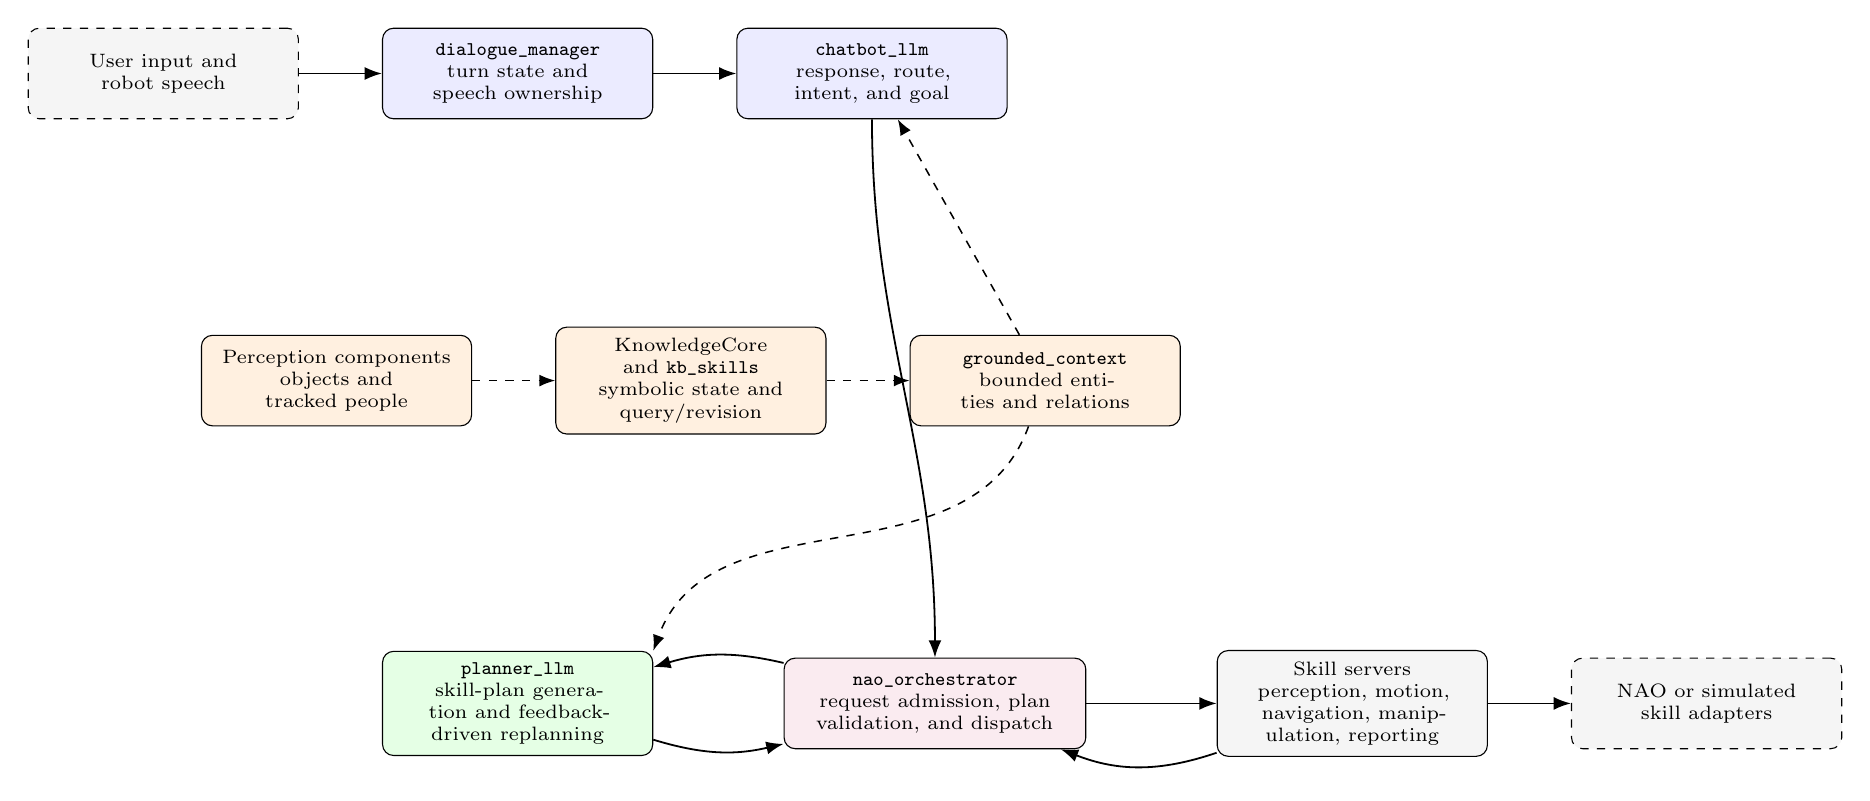
\begin{tikzpicture}[
  font=\scriptsize,
  >=Latex,
  component/.style={draw,rounded corners,align=center,text width=3.15cm,minimum height=1.15cm,inner sep=4pt},
  external/.style={component,dashed,fill=gray!8},
  dialogue/.style={component,fill=blue!8},
  planning/.style={component,fill=green!10},
  execution/.style={component,fill=purple!8},
  grounding/.style={component,fill=orange!12},
  flow/.style={-{Latex[length=2.2mm]},line width=0.65pt},
  evidence/.style={-{Latex[length=2.0mm]},line width=0.55pt,dashed}
]

\node[external] (user) at (-9.6,5.0) {User input and robot speech};
\node[dialogue] (dm) at (-5.1,5.0) {\code{dialogue_manager}\\turn state and speech ownership};
\node[dialogue] (chat) at (-0.6,5.0) {\code{chatbot_llm}\\response, route, intent, and goal};

\node[grounding] (perception) at (-7.4,1.1) {Perception components\\objects and tracked people};
\node[grounding] (kb) at (-2.9,1.1) {KnowledgeCore and \code{kb_skills}\\symbolic state and query/revision};
\node[grounding] (context) at (1.6,1.1) {\code{grounded_context}\\bounded entities and relations};

\node[planning] (planner) at (-5.1,-3.0) {\code{planner_llm}\\skill-plan generation and feedback-driven replanning};
\node[execution,text width=3.55cm] (orch) at (0.2,-3.0) {\textbf{\code{nao_orchestrator}}\\request admission, plan validation, and dispatch};
\node[component,fill=gray!8] (skills) at (5.5,-3.0) {Skill servers\\perception, motion, navigation, manipulation, reporting};
\node[external] (platform) at (10.0,-3.0) {NAO or simulated skill adapters};

\draw[flow] (user) -- (dm);
\draw[flow] (dm) -- (chat);
\draw[evidence] (perception) -- (kb);
\draw[evidence] (kb) -- (context);
\draw[evidence] (context) -- (chat);
\draw[evidence] (context) to[out=-110,in=70] (planner.north east);
\draw[flow] (chat.south) to[out=-90,in=90] (orch.north);
\draw[flow] (orch) to[bend right=15] (planner);
\draw[flow] (planner) to[bend right=15] (orch);
\draw[flow] (orch) -- (skills);
\draw[flow] (skills) -- (platform);
\draw[flow] (skills) to[bend left=20] (orch);

\end{tikzpicture}
\caption{Full-stack implementation of the modular interaction architecture. Dialogue interpretation and symbolic grounding provide the planner input; \code{nao_orchestrator} admits the request, validates the returned plan, dispatches skill servers, and forwards execution feedback. Robot-facing and simulated adapters share the same typed skill-result boundary.}
\label{fig:full-stack-implementation}
\end{figure}
\end{landscape}

\subsection{\code{dialogue_manager}}

\code{dialogue_manager} is the ROS~2 lifecycle component responsible for multimodal communication between the robot and its interlocutors. Following the upstream package design\footnote{Package source: \url{https://github.com/ieverythng/dialogue_manager}.}, it preserves chronological conversation histories for active interlocutors and associates incoming \code{hri_msgs/LiveSpeech} streams with the relevant dialogue state. The node invokes the chatbot through \code{DialogueInteraction}, exposes the high-level \code{/skill/chat}, \code{/skill/ask}, and \code{/skill/say} interfaces, and realises final user-facing expressions through the configured Say sub-skill.

This ownership boundary is also a runtime constraint. Planning and execution components publish structured communication requests through the designated dialogue interfaces, while \code{dialogue_manager} retains responsibility for the final utterance and its delivery through the speech backend.

Planner dialogue acts return through the same boundary. \code{planner_llm} publishes structured acknowledgement, clarification, failure, or completion acts on \path{/planner/dialogue_act}; \code{nao_orchestrator} relays the admitted act on \path{/nao_orchestrator/planner_dialogue_act}; and the dialogue layer selects the final wording and speech mechanism. This arrangement provides one user-facing speech authority for each semantic event and makes duplicate acknowledgements or completion reports observable during validation.

\subsection{\code{chatbot_llm}}

\code{chatbot_llm} is a lifecycle-managed semantic-routing node built on the existing chatbot scaffold. Its turn callback receives a \code{DialogueInteraction} request and the conversation history assembled by \code{dialogue_manager}. Before response generation or planner handoff, it queries the KB through \code{kb_skills}, reads the most recent \code{/scene/summary}, and passes both sources through the \code{PlannerHandoff} projection helper. The resulting \code{grounded_context}, defined by Contract~3, contains a bounded set of entities, locations, and task-relevant relations instead of raw detector streams or unrestricted KB rows. This projection informs dialogue and knowledge answers on every user turn and is attached to Contract~2 when the selected route produces a planner request.

The turn engine implements the route field from Contract~1 as follows:
\begin{itemize}
  \item A \code{dialogue} route covers conversational and task-discussion turns and does not publish planner work.
  \item A \code{knowledge_query} route answers from current symbolic evidence without causing a physical action. For example, ``what can you see?'' can use the current grounded context, whereas ``scan and tell me what you see'' requests fresh sensing and is eligible for execution.
  \item An \code{execution} route constructs planner-facing metadata such as goal text, request kind, normalised intent hints, and target KB entities. It publishes a candidate request to \code{/nao_orchestrator/planner_request} without constructing the skill sequence itself.
\end{itemize}

The chatbot prompt defines the component role, the permitted routes, the response requirements, and the structured intent fields. Runtime context adds the dialogue history, available skill summary, and grounded entities. In the evaluated \code{response_first} configuration, the first model call produces the acknowledgement and route decision; the intent stage then extracts goal and target metadata under that route. The \code{intent_first} ablation reverses the stage order and constrains response generation with the previously selected route. Both configurations produce the same Contract~1 output and planner-request format, which allows route consistency to be compared without changing downstream interfaces.

Figure~\ref{fig:chatbot-llm-node} summarises the implemented turn path and the two possible outputs: a response returned to the dialogue manager or an execution request submitted for planner admission.

\begin{figure}[H]
\centering
\resizebox{\textwidth}{!}{%
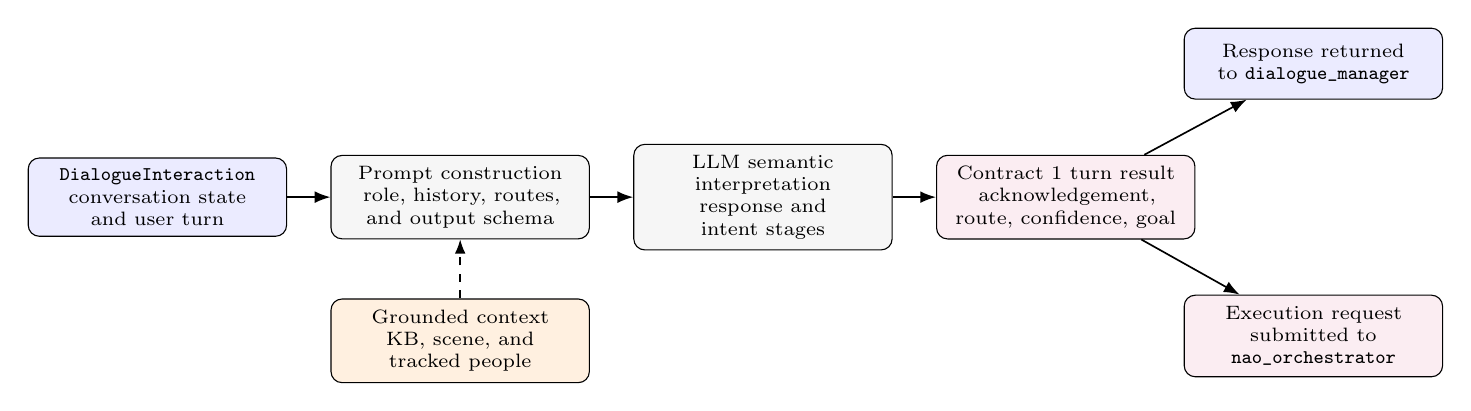
\begin{tikzpicture}[
  font=\scriptsize,
  >=Latex,
  node distance=0.55cm,
  box/.style={draw,rounded corners,align=center,text width=3.0cm,minimum height=0.9cm,inner sep=4pt},
  dialogue/.style={box,fill=blue!8},
  grounding/.style={box,fill=orange!12},
  process/.style={box,fill=gray!7},
  output/.style={box,fill=purple!7},
  arr/.style={-{Latex[length=2mm]},line width=0.6pt},
  support/.style={-{Latex[length=1.8mm]},line width=0.5pt,dashed}
]
\node[dialogue] (turn) {\code{DialogueInteraction}\\conversation state and user turn};
\node[process,right=of turn] (prompt) {Prompt construction\\role, history, routes, and output schema};
\node[process,right=of prompt] (model) {LLM semantic interpretation\\response and intent stages};
\node[output,right=of model] (result) {Contract~1 turn result\\acknowledgement, route, confidence, goal};
\node[grounding,below=0.75cm of prompt] (context) {Grounded context\\KB, scene, and tracked people};
\node[dialogue,above right=0.70cm and -0.15cm of result] (response) {Response returned to \code{dialogue_manager}};
\node[output,below right=0.70cm and -0.15cm of result] (handoff) {Execution request submitted to \code{nao_orchestrator}};
\draw[arr] (turn) -- (prompt);
\draw[arr] (prompt) -- (model);
\draw[arr] (model) -- (result);
\draw[support] (context) -- (prompt);
\draw[arr] (result) -- (response);
\draw[arr] (result) -- (handoff);
\end{tikzpicture}
}
\caption{Internal \code{chatbot_llm} path. Dialogue history and grounded context condition a structured semantic decision that either returns a user-facing response or submits an execution request for admission.}
\label{fig:chatbot-llm-node}
\end{figure}

\subsection{\code{planner_llm}}

\code{planner_llm} is the high-level planning node and contains a goal-keyed planning-state helper for feedback-driven state transitions. The node subscribes to admitted \code{/planner/request} messages instead of directly consuming chatbot output. Through \code{planner_common}, each request is normalised into the canonical contract with goal metadata nested under \code{plan}. The planner prompt combines the goal text, request kind, normalised intent hints, grounded context, the shared skill-entry projection from Contract~4, permitted step types, and the required JSON output envelope.

The planner prompt is assembled from the admitted request, bounded grounded entities, the skill-registry fields relevant to selection and ordering, the permitted step types, and the planner output contract. It specifies the available skills, required arguments, expected effects, observable completion evidence, and failure modes that may require clarification or replanning. This registry projection links the model's language-level proposal to the typed ROS~2 execution surface.

The model response remains a candidate until the planner engine extracts the JSON object, normalises its schema, validates the required metadata and step fields, and applies one bounded repair retry when configured. Unsupported skill names, malformed arguments, invalid recovery policies, or unparseable output become typed failure or clarification outcomes. Valid plans are published on \code{/intents} for independent orchestrator validation.

Evidence-producing plans receive an additional reporting check. When \code{report_result} follows a sensing, navigation, motion, or manipulation skill, \code{planner_common} requires the reporting step to omit planner-authored result wording. Compatibility normalisation removes fields such as \code{summary_text}, \code{result_summary}, \code{text}, \code{message}, and \code{utterance} before validation. The reporting step is later resolved from the preceding Contract~6 result payload, preventing an expected effect from being presented as an observed result.

The node also subscribes to \code{/planner/execution_feedback}. The embedded planning-state helper associates relevant events with the active goal and invokes the planning path when the orchestrator reports completion, failure, a recoverable condition, or a need for user input. The response may be a revised plan or a structured dialogue act. Robot control remains with the orchestrator, while user-facing communication follows the planner-dialogue relay and dialogue manager.

Figure~\ref{fig:planner-llm-node} shows the planner model call together with its validation, retry, feedback, and publication paths.

\begin{figure}[H]
  \centering
  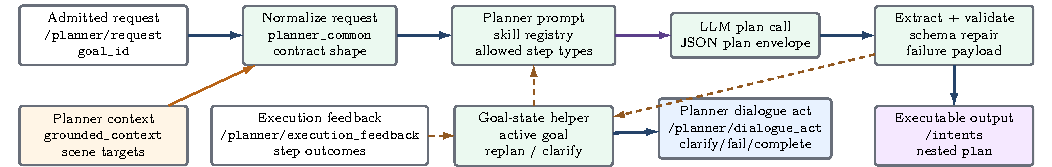
\includegraphics[width=\linewidth]{figures/chapter5_planner_llm.pdf}
  \caption{Internal \code{planner_llm} path, from admitted request through validated plan envelope and feedback-driven goal-state handling.}
  \label{fig:planner-llm-node}
\end{figure}

\subsection{Goal-Keyed Planning-State Helper}

The goal-keyed planning-state helper maintains planning state under an active \code{goal_id}. Each accepted plan carries a \code{plan_id} and monotonically meaningful \code{plan_version}; stable \code{step_id} values allow a newer plan version to preserve completed work when replanning continues the same goal. Feedback from an older or unrelated version is rejected before it can alter the current goal state.

The helper distinguishes planning, replanning, waiting-for-user, completed, and failed states. Step feedback may advance the goal, expose a recoverable condition, or produce a structured dialogue act. If a replacement plan is required, \code{planner_llm} creates and validates it under a newer version. Execution supervision and step dispatch remain within \code{nao_orchestrator}; the helper maintains planning order and lineage across these transitions.

\subsection{Skill Registry (\code{skill_common})}

The planner-facing capability model is derived from the canonical skill registry maintained by \code{skill_common}. Contract~4 and Table~\ref{tab:skill-entry-contract} define the shared entry shape: canonical name and aliases, typed parameters, preconditions, expected effects, observable success evidence, failure modes, result schema, safety flags, runtime availability, and executor mapping. The planner receives a bounded projection of these fields when it selects and orders skills. The orchestrator uses the same names, argument requirements, and availability information when it validates Contract~5 plans and dispatches Contract~6 calls. This arrangement provides a machine-checkable guard against divergence between the prompt-visible capability model and the execution surface.

Table~\ref{tab:runtime-skill-surface} lists the planner-visible skill set. Knowledge-base add, revise, and remove operations remain knowledge-service operations and are not included in this registry. Appendix~\ref{sec:runtime-skill-inventory} gives the arguments, expected evidence, failure modes, and executor for each entry.

\begin{table}[H]
\centering
\scriptsize
\renewcommand{\arraystretch}{1.16}
\caption{Planner-visible skills and their implementations.}
\label{tab:runtime-skill-surface}
\begin{tabularx}{\textwidth}{
@{}
>{\raggedright\arraybackslash}p{0.22\textwidth}
>{\raggedright\arraybackslash}X
>{\raggedright\arraybackslash}p{0.25\textwidth}
>{\raggedright\arraybackslash}p{0.13\textwidth}
@{}}
\toprule
\textbf{Skill} & \textbf{Purpose} & \textbf{Implementation} & \textbf{Controlled simulation}\\
\midrule
\code{scan} & Refresh scene evidence and return a typed scan payload. & First-party \code{/skill/scan} server. & Shared scene-fixture control.\\
\code{find_object} & Find one specified object and return whether it was found. & Perception or simulated adapter. & Yes.\\
\code{inspect_area} & Return the objects and people observed in a specified area. & Perception or simulated adapter. & Yes.\\
\code{navigate_to} & Reach a semantic destination such as a person, object, or location. & Navigation or simulated adapter. & Yes.\\
\code{walk_to} & Execute a short body-relative locomotion segment. & Robot movement or simulated adapter. & Yes.\\
\code{pick_object} & Grasp one specified object and return the observed result. & Manipulation or simulated adapter. & Yes.\\
\code{place_object} & Place a held object at a specified destination. & Manipulation or simulated adapter. & Yes.\\
\code{bring_object} & Deliver one specified object to a person or location. & Composite manipulation or simulated adapter. & Yes.\\
\code{perform_motion} & Execute a named body motion, including a greeting wave. & Motion replay or simulated adapter. & Yes.\\
\code{look_at} & Direct the robot's gaze towards a specified target. & Head, gaze, or simulated adapter. & Yes.\\
\code{ask_user} & Request information needed to continue planning. & Dialogue interface. & Trace-based.\\
\code{report_result} & Report an outcome derived from completed skill results. & Dialogue and reporting interface. & Trace-based.\\
\bottomrule
\end{tabularx}
\end{table}

\subsection{\code{nao_orchestrator} and Plan Execution}

\code{nao_orchestrator} implements deterministic execution of accepted plans. Before dispatch, it validates the plan envelope, ordered steps, registered skill names, arguments, dependencies, failure policies, and goal/plan lineage against the shared skill registry and runtime contracts. A plan is accepted only when every executable step can be resolved to an available skill interface.

Accepted plans are executed in order through the ROS action or skill-server interface mapped by each registry entry. The orchestrator retains the active goal, plan version, current step, completed results, and pending work. For each step it publishes the corresponding started, succeeded, or failed event on \code{/planner/execution_feedback}, preserving the identifiers required to associate execution evidence with the correct goal and plan version.

Each dispatched skill must return a typed Contract~6 result before the step can complete. Successful state-changing results may include world-state updates, which are applied through \code{kb_skills} and verified through a subsequent query when available. On failure, the orchestrator follows the validated step policy: it may stop the plan, continue only when permitted, or publish feedback that requests replanning or clarification. Replacement plans remain the responsibility of \code{planner_llm}.

Figure~\ref{fig:nao-orchestrator-node} summarises the validated plan-execution path described above.

\begin{figure}[H]
\centering
\resizebox{\textwidth}{!}{%
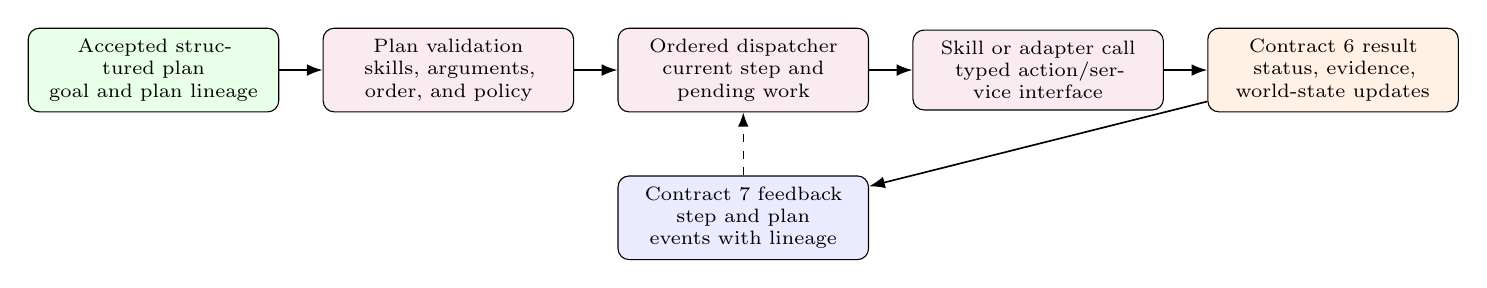
\begin{tikzpicture}[
  font=\scriptsize,
  >=Latex,
  node distance=0.55cm,
  box/.style={draw,rounded corners,align=center,text width=2.9cm,minimum height=0.95cm,inner sep=4pt},
  input/.style={box,fill=green!9},
  execution/.style={box,fill=purple!8},
  result/.style={box,fill=orange!11},
  feedback/.style={box,fill=blue!8},
  arr/.style={-{Latex[length=2mm]},line width=0.6pt},
  support/.style={-{Latex[length=1.8mm]},line width=0.5pt,dashed}
]
\node[input] (plan) {Accepted structured plan\\goal and plan lineage};
\node[execution,right=of plan] (validate) {Plan validation\\skills, arguments, order, and policy};
\node[execution,right=of validate] (dispatch) {Ordered dispatcher\\current step and pending work};
\node[execution,right=of dispatch] (skill) {Skill or adapter call\\typed action/service interface};
\node[result,right=of skill] (result) {Contract~6 result\\status, evidence, world-state updates};
\node[feedback,below=0.8cm of dispatch] (feedback) {Contract~7 feedback\\step and plan events with lineage};
\draw[arr] (plan) -- (validate);
\draw[arr] (validate) -- (dispatch);
\draw[arr] (dispatch) -- (skill);
\draw[arr] (skill) -- (result);
\draw[arr] (result) -- (feedback);
\draw[support] (feedback) -- (dispatch);
\end{tikzpicture}
}
\caption{Execution path implemented by \code{nao_orchestrator}. Accepted plans are validated, dispatched in order, and correlated with typed skill results and execution feedback.}
\label{fig:nao-orchestrator-node}
\end{figure}

\section{World State and Scene Grounding}

The perception path has parallel people and object branches. The person branch reuses \code{hri_face_detect_yunet}, \code{hri_person_manager}, and the ROS4HRI person interfaces to provide identities, tracked-person topics, and frame-qualified state \parencite{mohamed2020ros4hri}. The object branch uses \code{nao_scene_grounding} to convert detector output into a provider-independent scene representation. A custom YOLO detector was trained for a restricted proof-of-concept object set and integrated with the NAO camera stream through ROS. Its strongest demonstration classes are blueberry, corn, pear, tomato, and zucchini. Detector backends are normalised into one internal observation shape so that downstream components do not depend on the detector message type.

The grounding node filters object detections by confidence and an explicit label allowlist, maps labels to KB classes, and maintains local identifiers using tracker IDs or bounded image-plane matching. Without a tracker ID, the default matcher requires the same label, KB class, and detector source, a displacement of at most 64 pixels, and an observation age of at most two seconds. It publishes \code{/scene/summary} and writes accepted observations as transient KnowledgeCore statements through \code{/kb/revise}. Under the default configuration, KB observations have a four-second lifespan and are refreshed no more often than once per second; a local object is removed from the current scene summary after 4.5 seconds without a new detection. An object marked visible in \code{grounded_context} is therefore present in this bounded current-scene window. People remain managed by the tracked-person pipeline and are merged when compact symbolic context is assembled.

\code{kb_skills} provides the query and revision interface for KnowledgeCore. The chatbot formats a bounded query result as an internal knowledge snapshot, combines it with the current scene summary and tracked-person state, and emits the Contract~3 \code{grounded_context}. The projection retains entities, locations, and bounded relations while omitting unrestricted raw rows and detector payloads.

Planning context and execution evidence consequently have different roles. Current symbolic state supports knowledge answers and plan selection. Execution claims require a fresh Contract~6 result from the responsible skill. When \code{pick_object}, \code{place_object}, or \code{bring_object} changes the world state, the result identifies the corresponding removals and additions; the orchestrator reflects them through \code{kb_skills} and verifies the required postconditions when the query interface is available.

Figure~\ref{fig:perception-grounding-pipeline} presents the implemented object, person, knowledge, and compact-grounding paths.

\begin{figure}[H]
\centering
\resizebox{\textwidth}{!}{%
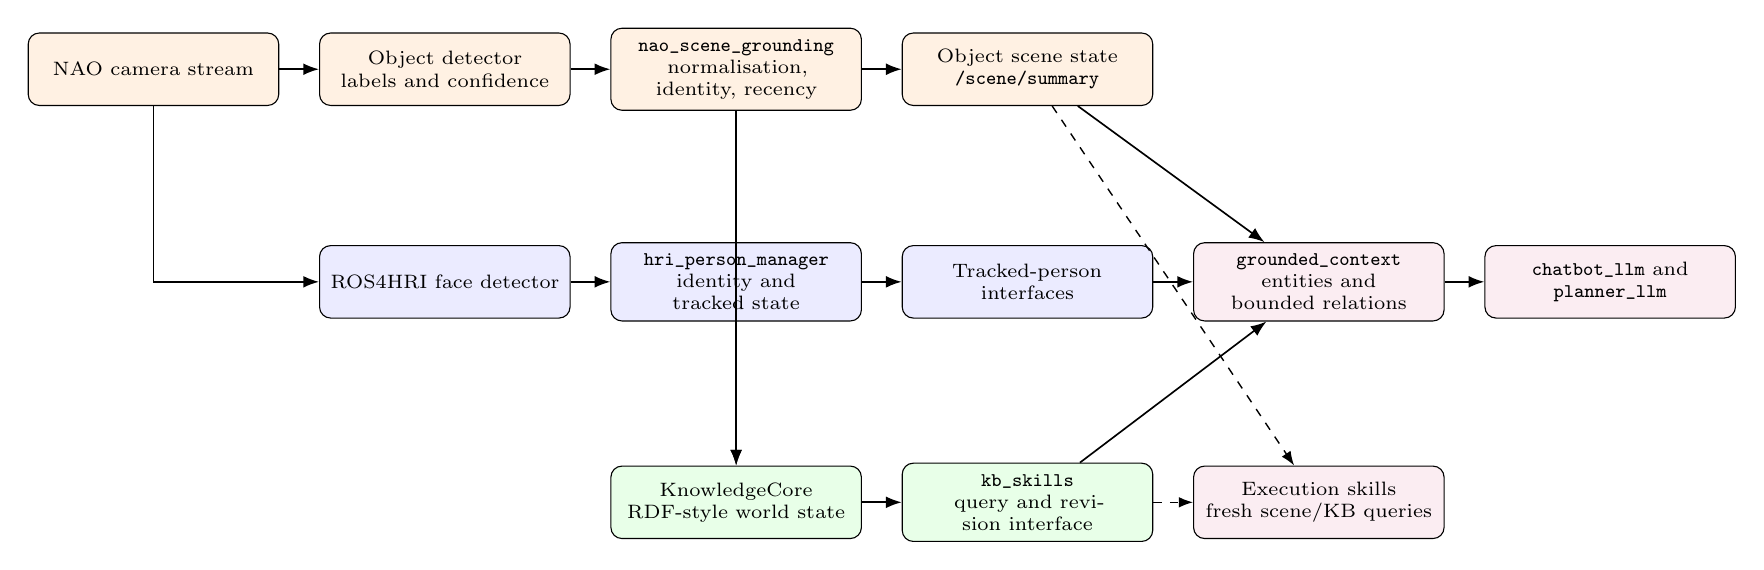
\begin{tikzpicture}[
  font=\scriptsize,
  >=Latex,
  box/.style={draw,rounded corners,align=center,text width=2.9cm,minimum height=0.92cm,inner sep=4pt},
  reused/.style={box,fill=blue!8},
  local/.style={box,fill=orange!11},
  knowledge/.style={box,fill=green!9},
  consumer/.style={box,fill=purple!7},
  arr/.style={-{Latex[length=2mm]},line width=0.6pt},
  support/.style={-{Latex[length=1.8mm]},line width=0.5pt,dashed}
]
\node[local] (camera) at (0,1.5) {NAO camera stream};
\node[local] (detector) at (3.7,1.5) {Object detector\\labels and confidence};
\node[local] (scene) at (7.4,1.5) {\code{nao_scene_grounding}\\normalisation, identity, recency};
\node[local] (summary) at (11.1,1.5) {Object scene state\\\code{/scene/summary}};

\node[reused] (face) at (3.7,-1.2) {ROS4HRI face detector};
\node[reused] (person) at (7.4,-1.2) {\code{hri_person_manager}\\identity and tracked state};
\node[reused] (personstate) at (11.1,-1.2) {Tracked-person interfaces};

\node[knowledge] (kc) at (7.4,-4.0) {KnowledgeCore\\RDF-style world state};
\node[knowledge] (kbskills) at (11.1,-4.0) {\code{kb_skills}\\query and revision interface};
\node[consumer] (context) at (14.8,-1.2) {\code{grounded_context}\\entities and bounded relations};
\node[consumer] (llm) at (18.5,-1.2) {\code{chatbot_llm} and \code{planner_llm}};
\node[consumer] (skills) at (14.8,-4.0) {Execution skills\\fresh scene/KB queries};

\draw[arr] (camera) -- (detector);
\draw[arr] (detector) -- (scene);
\draw[arr] (scene) -- (summary);
\draw[arr] (camera) |- (face);
\draw[arr] (face) -- (person);
\draw[arr] (person) -- (personstate);
\draw[arr] (scene) -- (kc);
\draw[arr] (person) -- (kc);
\draw[arr] (kc) -- (kbskills);
\draw[arr] (summary) -- (context);
\draw[arr] (personstate) -- (context);
\draw[arr] (kbskills) -- (context);
\draw[arr] (context) -- (llm);
\draw[support] (summary) -- (skills);
\draw[support] (kbskills) -- (skills);
\end{tikzpicture}%
}
\caption{Implemented perception and symbolic-grounding pipeline. Reused person-perception components and the local object-grounding path provide bounded scene and knowledge representations to dialogue, planning, and execution skills.}
\label{fig:perception-grounding-pipeline}
\end{figure}

\section{Skill Adapters and Controlled Simulation}

The implementation exposes the planner-visible capabilities in Table~\ref{tab:runtime-skill-surface} through a common adapter boundary. Robot-facing adapters invoke the available physical implementation, whereas the package named \code{fake_skills} supplies deterministic simulated action servers for controlled software evaluation. Both paths preserve the Contract~6 result shape. Simulated results additionally record \code{metadata.fake=true}, the scenario and result mode, the selected policy source, the deterministic seed when applicable, and the simulated duration. Dispatch and outcome events are published on \code{/fake_skills/events}.

The same planner and orchestrator path can therefore be exercised with physical results or with all-success, fail-once, and seeded pseudo-random simulated outcomes. Stateful policies use deterministic call counters and recorded seeds. Successful simulated results represent the corresponding world-state changes, which are reflected in KnowledgeCore so that later plan steps and dialogue turns observe the updated scenario rather than the initial fixture.

Controlled skill-adapter evidence supports software-level claims about route selection, plan validity, ordered dispatch, typed feedback, replanning, clarification, report coverage, and symbolic postconditions. Deterministic simulation also makes it possible to place a known failure at a selected execution step and observe whether the remaining goal is safely replanned. Physical navigation accuracy, grasp reliability, manipulation success, perception accuracy, NAOqi timing, and human-robot safety require separate embodied evaluation.

\section{Models and Runtime Configuration}

The implementation can run with the NAO adapters or deterministic simulated skill adapters while retaining the same dialogue, grounding, planning, orchestration, and result contracts. Model and backend selection are supplied through runtime configuration, so changing an inference provider does not require a different ROS~2 interface.

The primary evaluated configuration uses \code{Qwen3-VL-30B-A3B-Instruct-AWQ} for chatbot and planner inference through an OpenAI-compatible vLLM endpoint. The planner uses temperature \(0.1\) and an 800-token output bound. Additional Qwen3.5 and Ollama-hosted models were exercised over narrower evidence sets and are reported separately in Chapter~\ref{chap:results}.

Interface compatibility does not imply equivalent semantic behaviour. Model, backend, prompt version, sampling configuration, and token limits are therefore recorded as part of the experimental configuration and compared under the controls defined in Chapter~\ref{chap:validation-methodology}.

\chapter{Validation Methodology}
\label{chap:validation-methodology}

\section{Evaluation Aim}

The validation methodology is designed to test the thesis claim at the architectural level: a robot-facing LLM planner is useful only if its plans remain grounded in the live ROS4HRI state, respect the available skill contracts, expose execution failures through typed feedback, and produce user-facing dialogue through the intended speech owner. The evaluation therefore does not treat success as a single demonstration outcome. It treats success as a combination of route correctness, plan validity, execution supervision, recovery behaviour, and traceability.

The validation strategy is based on three evidence layers. The first layer is a controlled planner-request suite, where the planner receives deterministic requests with fixed grounded context. This isolates planning, schema compliance, and orchestrator dispatch from ASR and dialogue timing. The second layer is a full user-turn questionnaire, where utterances enter through the ROS4HRI speech path and therefore test dialogue routing, chatbot prompt behaviour, planner handoff, and exactly-once speech. The third layer is a fake-skill scenario suite, where deterministic skill outcomes are injected through the fake skill server to test success, failure, ambiguity, and recovery without depending on the physical robot.

\section{Validation Goals}

Table~\ref{tab:validation-goals-expanded} gives the validation goals used to score the system. These goals are deliberately operational. Each goal can be checked from ROS topic traces, planner JSON, fake-skill events, or container logs.

\begin{longtable}{p{0.23\linewidth}p{0.34\linewidth}p{0.32\linewidth}}
\toprule
\textbf{Goal} & \textbf{Question} & \textbf{Evidence source}\\
\midrule
\endfirsthead
\toprule
\textbf{Goal} & \textbf{Question} & \textbf{Evidence source}\\
\midrule
\endhead
Route correctness & Does the chatbot keep dialogue-only turns out of the planner and send execution-looking turns to the planner or orchestrator? & \code{/chatbot_llm/turn_trace}, \code{/intents}, \code{/planner/request}\\
Plan validity & Does the planner output valid JSON using admissible skill names, argument fields, and failure policies? & Planner output, \code{planner_common} normalisation, orchestrator validation\\
Skill coverage & Are all requested subgoals represented in the emitted plan, including composite instructions? & Plan steps, expected-plan checklist\\
Grounding use & Does the planner use \code{grounded_context}, \code{knowledge_snapshot}, \code{scene_summary}, and \code{state_t0} when a task depends on visible objects or people? & Planner request payload, KB query evidence, \code{/scene/summary}\\
Execution supervision & Does \code{nao_orchestrator} execute only validated steps and return structured feedback to the planner? & \code{/planner/execution_feedback}, orchestrator logs\\
Failure handling & Does a failure cause clarification, replanning, or safe termination rather than a false success message? & Fake-skill result payloads, planner dialogue acts\\
Exactly-once speech & Does one semantic event produce one user-facing response, without duplicated acknowledgement or completion speech? & \code{/planner/dialogue_act}, \code{/debug/nao_say/speech}, dialogue manager output\\
Trace completeness & Can each run be reconstructed from the saved JSONL trace and report bundle? & \code{interaction_trace_viewer}, \code{/fake_skills/events}, validation reports\\
\bottomrule
\caption{Validation goals for planner-mediated ROS4HRI execution.}
\label{tab:validation-goals-expanded}
\end{longtable}

\section{Questionnaire-Based Runtime Checks}

The runtime questionnaire complements the structured validation suite. Its purpose is to expose integration faults that planner-only tests can miss. Each item is marked as \emph{pass}, \emph{degraded}, \emph{fail}, or \emph{not run}. A failure in simple dialogue, duplicate speech, raw planner leakage, or false execution success is treated as a high-severity result because it directly affects user-visible behaviour.

\begin{longtable}{p{0.18\linewidth}p{0.32\linewidth}p{0.38\linewidth}}
\toprule
\textbf{Category} & \textbf{Representative prompt} & \textbf{Expected behaviour}\\
\midrule
\endfirsthead
\toprule
\textbf{Category} & \textbf{Representative prompt} & \textbf{Expected behaviour}\\
\midrule
\endhead
Simple dialogue & ``Hey'', ``How are you?'', ``What is your favourite colour?'' & The route remains dialogue-only, no planner request is emitted, and exactly one response is spoken.\\
Knowledge dialogue & ``What can you see?'', followed by a simulator object insertion and a repeated query & Newly inserted simulator or KB facts appear in \code{grounded_context} and are used in the answer.\\
Simple skill & ``Move your head to the right'', ``Wave at me'' & The system emits one acknowledgement, dispatches one skill, and reports truthful completion or failure.\\
Composite skill & ``Navigate to the phone and tell me what else you see'' & The planner emits ordered steps, preserves intermediate evidence, and reports the complete chain.\\
Simple fake skill & \code{find_object(cup)} under success, ambiguity, and failure modes & Fake payloads include \code{metadata.fake=true}, stable result modes, and recoverable failure fields where appropriate.\\
Composite fake skill & Multi-step navigation, search, and report under controlled fake outcomes & Completed steps are not repeated unnecessarily, failed steps are explained, and clarification is routed through dialogue.\\
\bottomrule
\caption{Tailored runtime questionnaire used for end-to-end validation.}
\label{tab:runtime-questionnaire}
\end{longtable}

\section{Fake-Skill Scenario Validation}

The fake-skill suite is the primary deterministic validation substrate. It avoids the main weakness of purely prompt-based simulation: the planner and orchestrator still interact with a ROS package that returns typed skill payloads, emits events, and can be configured at runtime. The fake-skill package supports global modes such as \code{scenario}, \code{always_success}, \code{always_fail}, \code{every_other}, and \code{random_seeded}. It also supports named scenarios such as \code{ambiguous_cup}, \code{path_blocked}, \code{social_wave_unavailable}, and \code{area_person_found}.

The scenario suite is organised around case families rather than isolated commands. This makes it possible to compare planner behaviour under different outcome policies while keeping the user goal fixed.

\begin{longtable}{p{0.17\linewidth}p{0.22\linewidth}p{0.27\linewidth}p{0.23\linewidth}}
\toprule
\textbf{Case family} & \textbf{Skill path} & \textbf{Outcome policies} & \textbf{Expected response}\\
\midrule
\endfirsthead
\toprule
\textbf{Case family} & \textbf{Skill path} & \textbf{Outcome policies} & \textbf{Expected response}\\
\midrule
\endhead
Object search & \code{find_object} & Found, not found, ambiguous, backend unavailable & Report object evidence, ask clarification when ambiguous, or explain failure.\\
Navigation & \code{navigate_to} or \code{walk_to} & Success, path blocked, unknown location, timeout & Continue on success, ask for alternative or safe stop on recoverable failure.\\
Perception and reporting & \code{scan -> report_result} & Success, empty scene, backend failure & Fill report from payload when available and avoid unsupported claims.\\
Social gesture & \code{look_at -> wave_greet} & Success, motion unavailable, safety disabled & Execute only admissible steps and explain social-motion failure.\\
Area inspection & \code{inspect_area} or \code{navigate_to -> scan -> report_result} & Clear, object found, person found, ambiguous area & Report observed area state or request clarification.\\
Composite instruction & Ordered mix of navigation, search, and reporting & All success, first failure, middle failure, alternating failure & Preserve step order, stop or replan safely, and summarise completed work.\\
\bottomrule
\caption{Scenario matrix for deterministic fake-skill validation.}
\label{tab:fake-skill-scenario-matrix}
\end{longtable}

\section{Deep Fake-Skill Scenario Blocks}

The term \emph{deep fake-skill scenario} is used here to mean a multi-step fake execution scenario with structured state, deterministic failure injection, and trace-level evidence. It is not a synthetic-media or deepfake-video component. These scenarios are important because many planner failures only appear after the first step has succeeded and the stack must decide whether to continue, replan, ask the user, or stop.

Three deep scenario blocks are used in the thesis evaluation design:

\begin{enumerate}
  \item \textbf{Ambiguous object recovery.} The user asks the robot to find or move toward ``the cup'' while the fake scene contains two cup candidates. The expected behaviour is not to choose arbitrarily. The planner should request clarification or produce a safe blocked outcome.
  \item \textbf{Path-blocked navigation.} The user asks the robot to navigate to a target. The fake skill returns \code{path_blocked} with \code{recoverable=true}. The expected behaviour is a replan, an alternative-route question, or a clear explanation that the path is blocked.
  \item \textbf{Composite report after execution.} The user asks the robot to visit or inspect several targets and report after each stage. The expected behaviour is an ordered plan, one feedback event per executed step, and a final response that reflects all completed and failed stages rather than only the last event.
\end{enumerate}

\section{Primary and Secondary Execution Modes}

The primary validation mode is planner-request injection. A controlled payload is published to the planner or planner-gate seam with fixed \code{goal_text}, \code{normalized_intents}, \code{scene_targets}, and \code{grounded_context}. This mode is fast and isolates the planner, orchestrator, and fake skill server.

The secondary validation mode is full user-turn injection. A user utterance is published through the ROS4HRI speech ingress, normally \code{/nao_chatbot/humans/voices/anonymous_speaker/speech}, after the corresponding speaker id has been published on the tracked voices topic. This mode is slower and more sensitive to runtime load, but it tests the chatbot route, dialogue manager handoff, and speech ownership.

\section{Metrics}

For each run, the validation log records the case id, utterance, route mode, fake-skill mode, scenario id, seed, planner call status, plan steps, dispatched skills, result statuses, clarification flag, final status, final response text, timeout flag, warning count, and error count. The main aggregate metrics are:

\begin{itemize}
  \item route accuracy;
  \item valid-plan rate;
  \item expected-skill coverage;
  \item fake-skill dispatch rate;
  \item safe-failure rate;
  \item clarification rate when ambiguity is expected;
  \item timeout rate;
  \item forbidden-plan rate, especially executable \code{say} steps when speech should remain under dialogue ownership;
  \item mean and maximum latency, when timestamps are available.
\end{itemize}

\section{Evidence Bundle}

A complete validation run should produce a reproducible bundle containing the suite configuration, JSONL trace, per-case metrics, aggregate metrics, and a short report. The expected layout is:

\begin{lstlisting}[style=sharedCode, caption={Expected validation evidence bundle.}]
docs/evaluation/runs/<timestamp>/
  suite_config.yaml
  trace.jsonl
  per_case_metrics.csv
  aggregate_metrics.json
  report.md
  report.html
  selected_traces/
    <case_id>_trace.json
\end{lstlisting}

The thesis uses this structure as the evidence contract. Results are considered preliminary when they come from focused runtime probes rather than a full repeated suite.

\chapter{Results}
\label{chap:results}

\section{Evidence Selection}

Each evidence set fixes its launch mode, model or source configuration, case set, artifact, and 1--10 run score. Scores from different tuples are not averaged because a model can produce fluent dialogue while reducing planner-schema validity or recovery reliability.

The evaluation contains four evidence sets. The 28 June response-first run supplies the broad full-stack baseline. The 8 July response-first run supplies the deterministic fake/replan matrix under JSON-only grounded context. The 10 July audit applies stricter KB-effect and report-result checks. The 11 July run is an alternate-model ablation and is reported separately from the principal configuration.

\begin{table}[H]
\centering
\small
\renewcommand{\arraystretch}{1.15}
\caption{Run-level evidence sets and reviewer scores.}
\label{tab:run-level-evidence}
\begin{tabularx}{\textwidth}{@{}p{0.12\textwidth}p{0.20\textwidth}p{0.16\textwidth}X p{0.08\textwidth}@{}}
\toprule
\textbf{Run} & \textbf{Profile} & \textbf{Scope} & \textbf{Evidence summary} & \textbf{Score}\\
\midrule
F28 & \code{response_first} & Full runtime & Speech ingress, KB add/revise/remove, simple and composite skills, grouped delivery, direct fake guards, and KB post-effects. & 8.7\\
F08 & \code{response_first}, JSON-only grounding & Fake/replan & Four eight-case deterministic policy sweeps through ROS4HRI speech ingress, with isolated confirmation probes. & 8.6\\
F10 & Strict seam audit & KB/report holdout & Natural KB mutation, grouped delivery effects, follow-up state, and replan/report checks. & 6.7\\
F11 & Alternate-model ablation & Main plus fake/replan & Fluent main questionnaire output, followed by planner-schema and deterministic-recovery regressions. & 5.8\\
\bottomrule
\end{tabularx}
\end{table}

F28 and F08 are recorded in the full-suite and deterministic-fake-suite validation ledgers, including the source artifact identifiers and case-level assessments. F10 and F11 are preserved as the repository reports \path{runtime_review_2026-07-10_sv_seams.md} and \path{runtime_review_2026-07-11_qwen_personal_stack.md}. The scores in Table~\ref{tab:run-level-evidence} are the reviewer summaries recorded with those evidence sets; case counts and seam-level observations remain the primary quantitative results. The final evidence bundle described in Chapter~\ref{chap:validation-methodology} assigns these records stable run identifiers and hashes rather than relying on temporary runtime paths.

\section{Full ROS4HRI Runtime Results}

F28 exercised the response-first speech path from tracked voice and \code{LiveSpeech} through dialogue, planning, deterministic execution, feedback, and final speech. Table~\ref{tab:full-runtime-results} reports the principal seams retained from that run.

\begin{table}[H]
\centering
\small
\renewcommand{\arraystretch}{1.14}
\caption{Full-runtime results for evidence set F28.}
\label{tab:full-runtime-results}
\begin{tabularx}{\textwidth}{@{}p{0.24\textwidth}p{0.13\textwidth}X@{}}
\toprule
\textbf{Validation seam} & \textbf{Result} & \textbf{Observed evidence}\\
\midrule
Dialogue routing & Pass & Simple dialogue and informational turns remained outside planner execution and produced one user-facing response.\\
Stable KB query & Pass & Injected cup name, colour, and support relation were available through KB query, grounded context, and dialogue.\\
Explicit KB mutation & Pass & Structured add, revise, query, and remove traversed the planner/orchestrator KB boundary; the post-remove query was empty.\\
Simple skill & Pass & Head motion and wave cases reached registered execution paths and evidence-derived reporting.\\
Composite skill & Pass & Head-motion plus wave and ordered multi-object navigation/report produced ordered plans and terminal reports.\\
Grouped semantic execution & Pass & Kitchen objects and the named recipient were represented in planner work without fabricated detector evidence.\\
Fake skill guards & Pass & Canonical targets succeeded and absent or non-canonical targets returned typed failures.\\
Exactly-once speech & Pass & The retained speech traces contained no duplicated acknowledgement or terminal semantic event.\\
\bottomrule
\end{tabularx}
\end{table}

The run score of 8.7 reflects broad success across dialogue, grounding, execution, and KB transport while keeping detector object recognition outside the semantic-stack score. The score does not combine detector variability with KB-authored object grounding.

\section{Deterministic Fake-Skill and Replan Results}

Evidence set F08 used \code{response_first}, disabled the compact grounded-context digest, and exercised the same ROS4HRI speech ingress under four deterministic fake policies. Table~\ref{tab:fake-policy-results} reports the full-ladder result and the isolated confirmation result separately.

\begin{table}[H]
\centering
\small
\renewcommand{\arraystretch}{1.14}
\caption{Deterministic fake-skill policy results for evidence set F08.}
\label{tab:fake-policy-results}
\begin{tabularx}{\textwidth}{@{}p{0.23\textwidth}p{0.16\textwidth}p{0.18\textwidth}X@{}}
\toprule
\textbf{Policy} & \textbf{Full ladder} & \textbf{Isolated probe} & \textbf{Interpretation}\\
\midrule
\path{all_success} & 8/8 pass & Not required & Inventory, ordered reports, grouped delivery, maximal delivery, and multi-turn follow-up completed.\\
\path{fail_once_navigation} & 8/8 pass & Not required & Failed navigation produced a newer plan version or truthful recovery without duplicate active goals.\\
\path{fail_once_pick} & 7/8 pass & Failed ordered-report case passed in isolation & Recovery was correct outside the full-ladder context; the full-ladder result remains 7/8.\\
\path{delivery_blocked} & 6/8 pass & Gold-apple case passed; ordered report remained failed & Delivery failure was generally truthful, but case interaction affected ordered-target extraction.\\
\bottomrule
\end{tabularx}
\end{table}

The four full sweeps produced 29 passes from 32 cases. Severe fallback markers remained zero: no duplicate active goal, invalid planner JSON, invalid executable plan, backend-unreachable speech, execution-report fallback, or rules-response fallback was recorded in the selected run. The run-level reviewer score was 8.6. Isolated passes are retained as diagnostic evidence and do not replace the corresponding full-ladder failures.

The F08 ledger records one artifact for each policy sweep and separate artifacts for the isolated ordered-report and blocked-delivery probes. Keeping the full-sweep and isolated records distinct prevents a diagnostic pass from replacing the primary 29/32 result.

\section{Strict KB-Effect and Reporting Audit}

F10 applied stricter post-condition checks than the broad success-path run. The focused ordered-walk, grouped work-table delivery, missing-object recovery, and missing-recipient clarification cases passed under \code{all_success}; \code{fail_once_navigation} also showed failed navigation, replanning, and completed recovery. The run score was reduced to 6.7 because grouped kitchen delivery reported only one delivered object, a follow-up answer retained the cup in the kitchen, and direct KB queries exposed stale source-location facts and recipient-side object-like spatial predicates.

This result distinguishes execution completion from state correctness. A successful action result is insufficient when the verified post-state still contains mutually inconsistent location relations. The finding supports the use of Contract~6 KB effects, post-query verification, and a separate state-freshness metric.

\section{Alternate-Model Ablation}

F11 evaluated \code{qwen36-turbo-hermes} with response-first routing and JSON-only grounded context. The twenty-case main questionnaire was marked 20/20 pass and produced fluent dialogue. The deterministic fake/replan artifacts contained 38 scored case records: 22 pass, 7 degraded, and 9 fail. The post-run snapshot recorded nine deduplicated planner-invalid-JSON events, nine invalid executable-plan events, six planner-gate rejections, and 53 route-repair events.

\begin{table}[H]
\centering
\small
\caption{Alternate-model ablation results for evidence set F11.}
\label{tab:model-ablation-results}
\begin{tabularx}{\textwidth}{@{}p{0.25\textwidth}p{0.18\textwidth}X@{}}
\toprule
\textbf{Measure} & \textbf{Result} & \textbf{Interpretation}\\
\midrule
Main questionnaire & 20/20 pass & Response fluency and broad route behaviour were strong.\\
Fake/replan records & 22 pass, 7 degraded, 9 fail & Structured planning and recovery reliability regressed under deterministic policies.\\
Planner invalid JSON & 9 events & Fluent acknowledgement did not imply a valid executable plan.\\
Invalid executable plan & 9 events & Deterministic validation prevented malformed work from reaching skill dispatch.\\
Planner-gate rejection & 6 events & Admission guards remained observable under model pressure.\\
Route repair & 53 events & The turn engine frequently reconciled model route inconsistencies.\\
Reviewer score & 5.8/10 & Critical structured-output and recovery failures outweighed the fluent main-suite surface.\\
\bottomrule
\end{tabularx}
\end{table}

The ablation demonstrates why the 1--10 score and the fake/replan matrix are reported alongside questionnaire pass counts. A model that answers well at the dialogue surface may still impose substantial planner repair and validation pressure.

\section{ROS4HRI Contract Preservation}

Table~\ref{tab:ros4hri-results} summarises the architecture checks applied across the response-first evidence.

\begin{table}[H]
\centering
\small
\renewcommand{\arraystretch}{1.14}
\caption{ROS4HRI and runtime-contract results.}
\label{tab:ros4hri-results}
\begin{tabularx}{\textwidth}{@{}p{0.27\textwidth}p{0.14\textwidth}X@{}}
\toprule
\textbf{Contract check} & \textbf{Result} & \textbf{Evidence}\\
\midrule
Tracked voice and speech ingress & Pass & Scored speech cases entered through tracked voice and per-voice \code{LiveSpeech} with the dialogue manager active.\\
Dialogue and speech ownership & Pass & Planner dialogue crossed the orchestrator relay; no selected run contained duplicate semantic speech or raw planner text.\\
Planner admission ownership & Pass & Execution requests crossed the orchestrator planner gate before planner consumption.\\
Deterministic execution boundary & Pass & Invalid plans were observable as validation or gate events rather than direct robot dispatch.\\
Skill actions and feedback lineage & Pass & Fake/replan traces retained goal, plan version, step results, terminal evidence, and speech evidence.\\
KB transport ownership & Pass & Explicit mutations traversed \code{kb_skills}; ordinary questions did not mutate the KB.\\
Post-skill KB consistency & Degraded in F10 & Stale and recipient-side spatial predicates remained after one grouped-delivery configuration.\\
Detector profile separation & Pass & Detector object recognition was excluded from the semantic-stack score and retained as a separate profile.\\
\bottomrule
\end{tabularx}
\end{table}

\section{Result Synthesis}

The response-first evidence supports three conclusions. First, the architecture can preserve dialogue, planning, execution, and speech ownership while completing grounded simple and composite tasks. Second, deterministic fake policies provide stronger evidence than all-success demonstrations because they expose replan lineage, clarification, and truthful terminal behaviour. Navigation recovery was stable in F08, while manipulation and blocked-delivery profiles were more sensitive to full-ladder context. Third, surface fluency is not an adequate proxy for planner reliability. The alternate-model run passed the main questionnaire but produced substantially more invalid planner output and recovery failures.

The strict KB audit also shows that action success and state correctness must be reported separately. Contract~6 evidence and a terminal speech event can coexist with stale KB relations unless post-effects are verified. For that reason, Chapter~\ref{chap:validation-methodology} treats post-query state freshness, trace completeness, and exactly-once speech as independent acceptance dimensions rather than optional diagnostics.

\chapter{Discussion}
\label{chap:discussion}

\section{Architectural Findings}

The implementation and runtime traces show that modular planning can be inspected at boundaries that are absent from a prompt-to-action design. The planner does not own robot execution, speech output, or raw perception. It receives structured requests and returns structured plans or dialogue acts. Direct atomic execution was retained as an orchestrator control seam, but it was not treated as a matched experimental baseline because its capability scope differs from multi-step planner mediation.

The most useful architectural seam is the boundary between \code{planner_llm} and \code{nao_orchestrator}. The planner can propose a sequence, but the orchestrator validates and dispatches it. This makes it possible to test the planner with fake skills, physical skills, or unavailable skills without changing the planner prompt itself. It also means that execution feedback can be represented as a first-class input to replanning rather than as an unstructured error message.

\section{Planner Behaviour}

The planner design is strongest when the task can be represented as a sequence of available skill contracts. Atomic commands, object search, navigation, and report-generation tasks map naturally to the registry. Composite instructions are harder because they require the planner to preserve order, carry evidence between steps, and decide whether a later step should still run after an earlier failure.

The deterministic failure profiles showed that recovery quality depends on both feedback lineage and the availability of a semantically different valid plan. Navigation fail-once cases produced newer plan versions and truthful closure in the strongest historical sweep. Pick and blocked-delivery cases were less stable, and some later traces reached a safe stop without a complete post-terminal report. The planner can therefore react to feedback, but the evidence does not support a general recovery guarantee.

\section{Grounding and World State}

Grounding remains a central limitation. The architecture distinguishes compact prompt context, the detector-derived scene summary, and raw KB evidence because each has a different role. The chatbot needs a bounded world-state projection, the planner needs actionable entity identifiers and targets, and operators need traceable source evidence. The F13 semantic audit showed that presence in the projection is insufficient when target roles are not preserved through selection, planning, dispatch, and reporting.

The stable KB insertion probes separated fact availability from model use. Name, colour, support, and count queries passed in broad runs, while grouped post-effect queries exposed stale location relations after apparent delivery success. Action completion and state correctness must therefore be evaluated independently. This distinction also prevents detector variability from being misclassified as a planner or semantic-grounding failure.

\section{ROS4HRI Modularity}

The stack is partly robot-agnostic and partly NAO-specific. The planner request, planner output, execution feedback, and dialogue act contracts are not inherently tied to NAO. The same architecture could be reused with another ROS-compatible platform if an equivalent skill registry and orchestrator adapter were provided. By contrast, speech execution, replay motion, posture control, head motion, and look-at behaviour depend on NAO-specific packages or adapters.

This separation is a practical strength. It allows the thesis to evaluate the planner loop independently from the physical robot while still preserving a credible path to robot execution. The fake-skill layer is especially valuable because it provides deterministic execution evidence while the physical skills remain subject to hardware, safety, and perception variability.

\section{Validation Implications}

The difference between the F13 trajectory result and semantic audit is the main methodological finding. A case can contain speech ingress, planner admission, execution feedback, a terminal marker, and final speech while still acting on the wrong targets. Full user-turn injection remains necessary for route correctness, dialogue ownership, and exactly-once speech. Planner and action-level probes remain useful for isolating plan admission and skill guards. Neither is sufficient without an oracle that compares requested, selected, planned, executed, and reported members and then verifies the resulting KB state.

The runtime-review index is useful for operational triage, but it is secondary to explicit denominators and acceptance rules. The earlier 8.2 assessment and later 6.0 cap describe different evidence depths rather than a uniform performance decline. Reporting both makes the change in theorem strength visible instead of suppressing a safety finding to preserve a headline score.

\chapter{Limitations and Future Work}
\label{chap:limitations-future-work}

\section{Current Limitations}

The current system has several limitations. The physical implementation is centred on NAO, so cross-robot portability is architectural rather than fully proven. LLM planning remains sensitive to prompt design, model availability, token limits, and JSON schema adherence. The validation strategy is scenario-based and cannot prove exhaustive safety. Perception and grounding quality also constrain planner performance because a correct planner cannot reliably act on objects that are missing, stale, or ambiguously represented in the world state.

The current evidence base is also incomplete. The fake-skill substrate has been validated for selected deterministic action-level scenarios, but the full repeated planner-level suite still needs to be run. The user-turn path has shown degraded trace continuity in at least one live-stack pass. The planner request-admission path after clarification requires further focused testing.

\section{Future Work}

Future work should stabilise the planner-gate and goal-state transitions, then run the full fake-skill validation suite with repeated seeds and saved evidence bundles. The next implementation step is to make per-case metrics and aggregate reports a routine output of validation rather than a manual analysis product.

The architecture should also be extended in four directions: richer grounding through a persistent world model, broader skill-registry generation from reviewed contracts, safer composite and macro-skill execution, and cross-platform validation on another ROS-compatible robot or simulator. A longer-term extension would integrate a World Model Enricher that tracks uncertainty, object identity, and temporal freshness explicitly rather than passing only a compact snapshot to the planner.

\chapter{Conclusion}
\label{chap:conclusion}

This thesis has presented the design and implementation of a modular LLM-based planner for a ROS4HRI-compatible NAO robot stack. The central architectural decision is to keep dialogue, grounding, planning, deterministic execution, and speech ownership separated by explicit runtime contracts. This separation allows the planner to use natural-language reasoning while the robot-facing stack continues to validate skill names, arguments, execution feedback, and dialogue acts through inspectable ROS interfaces.

The implementation demonstrates how a chatbot can route execution-looking turns to a planner, how the planner can produce structured plans over a skill registry, and how an orchestrator can act as the execution boundary between generated plans and robot or fake-skill adapters. The runtime contracts make the system more auditable than a direct prompt-to-action design because planner requests, grounded context, generated plans, execution feedback, and dialogue acts can be captured and checked independently.

The preliminary validation evidence supports the usefulness of the fake-skill substrate for controlled evaluation. Deterministic scenarios for ambiguous object search, blocked navigation, and unavailable social motion returned the expected structured failure codes. These results make it possible to evaluate recovery behaviour without depending on physical robot variability. The same validation pass also exposed integration risks in repeated planner request admission and full user-turn trace continuity. These are useful findings because they identify the remaining runtime seams that must be stabilised before the system can be assessed as a complete end-to-end HRI planner.

Overall, the work supports a measured conclusion: LLM planning can be integrated into ROS4HRI more safely when it is constrained by symbolic context, skill contracts, deterministic orchestration, and structured feedback. The approach does not remove the need for careful runtime validation, but it gives that validation clear seams and reproducible evidence.


\appendix
\chapter{Full Runtime Contracts}
\label{chap:appendix}

The full runtime contracts are described in Chapter~\ref{chap:runtime-contracts}. This appendix is reserved for additional machine-readable schemas when the final validation artefacts are frozen.

\section{Runtime Skill Inventory}
\label{sec:runtime-skill-inventory}

Table~\ref{tab:runtime-skill-inventory} gives the compressed runtime projection used by the current planner and orchestrator profiles. The values are taken from the shared skill registry and are shortened only to fit the appendix. The machine-readable registry and the generated runtime projections are frozen with the source revision of each validation bundle. \code{ask_user} is retained as a planner dialogue act under Contract~7 and is not included in this execution-skill inventory.

\begin{longtable}{
>{\raggedright\arraybackslash}p{0.15\textwidth}
>{\raggedright\arraybackslash}p{0.14\textwidth}
>{\raggedright\arraybackslash}p{0.20\textwidth}
>{\raggedright\arraybackslash}p{0.25\textwidth}
>{\raggedright\arraybackslash}p{0.18\textwidth}}
\caption{Compressed runtime skill inventory and registry values.}\label{tab:runtime-skill-inventory}\\
\toprule
\textbf{Skill and category} & \textbf{Required parameters} & \textbf{Expected effect or evidence} & \textbf{Known failure modes} & \textbf{Executor and status}\\
\midrule
\endfirsthead
\multicolumn{5}{l}{\small\itshape Table~\thetable\ continued}\\
\toprule
\textbf{Skill and category} & \textbf{Required parameters} & \textbf{Expected effect or evidence} & \textbf{Known failure modes} & \textbf{Executor and status}\\
\midrule
\endhead
\midrule
\multicolumn{5}{r}{\small\itshape Continued on next page}\\
\endfoot
\bottomrule
\endlastfoot

\code{scan}\\ perception
& none
& refreshed scene evidence and typed scan payload
& \code{no_person}, \code{objects_only}, \code{backend_unavailable}, \code{unexpected_payload}
& \code{nao_orchestrator.scan}; first-party\\

\code{find_object}\\ perception
& \code{target}
& object or person evidence is returned
& \code{not_found}, \code{ambiguous}, \code{backend_unavailable}
& \code{fake_skills.find_object}; fake\\

\code{navigate_to}\\ navigation
& \code{target}
& robot arrives at the target location
& \code{path_blocked}, \code{unknown_location}, \code{safety_disabled}
& \code{fake_skills.navigate_to}; fake\\

\code{walk_to}\\ navigation
& none
& short local walking segment is executed or dry-run
& \code{invalid_local_goal}, \code{safety_disabled}, \code{path_blocked}, \code{naoqi_move_failed}
& \code{nao_orchestrator.walk_to}; hybrid\\

\code{bring_object}\\ manipulation
& \code{target}, \code{recipient}
& object is delivered to recipient or destination
& \code{acquisition_failure}, \code{navigation_failure}, \code{delivery_blocked}, \code{recipient_unavailable}
& \code{fake_skills.bring_object}; fake\\

\code{place_object}\\ manipulation
& \code{target}, \code{destination}
& object is released and a support relation is added
& \code{destination_unavailable}, \code{invalid_support}, \code{no_held_object}, \code{placement_failed}
& \code{fake_skills.place_object}; fake\\

\code{pick_object}\\ manipulation
& \code{target}
& robot holds the object and updates its support relation
& \code{object_unavailable}, \code{unreachable}, \code{already_held}, \code{grasp_failed}
& \code{fake_skills.pick_object}; fake\\

\code{perform_motion}\\ embodiment
& \code{object}
& robot posture or head orientation changes
& \code{unsupported_motion}, \code{dispatch_failed}
& \code{nao_orchestrator.perform_motion}; first-party\\

\code{look_at}\\ attention
& none
& robot gaze is redirected or reset
& \code{missing_target}, \code{dispatch_failed}
& \code{nao_orchestrator.look_at}; first-party\\

\code{kb_add}\\ knowledge
& \code{statements}
& requested predicates are added through KnowledgeCore
& \code{missing_statements}, \code{kb_service_unavailable}, \code{kb_mutation_rejected}
& \code{nao_orchestrator.kb_add}; first-party\\

\code{kb_revise}\\ knowledge
& \code{statements}
& requested predicates are revised through KnowledgeCore
& \code{missing_statements}, \code{kb_service_unavailable}, \code{kb_mutation_rejected}
& \code{nao_orchestrator.kb_revise}; first-party\\

\code{kb_remove}\\ knowledge
& \code{statements}
& requested predicates are removed through KnowledgeCore
& \code{missing_statements}, \code{kb_service_unavailable}, \code{kb_mutation_rejected}
& \code{nao_orchestrator.kb_remove}; first-party\\

\code{report_result}\\ communication
& none
& user receives a result summary through robot speech
& \code{missing_summary}, \code{say_dispatch_failed}
& \code{nao_orchestrator.report_result}; first-party\\

\code{wave_greet}\\ social motion
& none
& robot performs a greeting wave gesture
& \code{motion_unavailable}, \code{safety_disabled}, \code{unexpected_payload}
& \code{nao_orchestrator.wave_greet}; hybrid\\

\code{inspect_area}\\ perception
& \code{target}
& scene evidence for the target area is returned
& \code{ambiguous}, \code{area_unknown}, \code{backend_unavailable}
& \code{fake_skills.inspect_area}; fake\\

\end{longtable}

The inventory separates the planner-facing name from the executor mapping. It also records whether failure injection is supported in the current fake profile, which is used by the multi-step deterministic fake-skill cases in Chapter~\ref{chap:validation-methodology}. The table does not imply that every hybrid or fake entry is enabled in the primary scored launch profile.

\chapter{Launch Commands}

\begin{lstlisting}[style=sharedCode]
ros2 launch nao_chatbot nao_chatbot_sim_demo.launch.py \
  start_planner_llm:=true \
  chatbot_planner_mode_enabled:=true \
  planner_llm_think:=false
\end{lstlisting}

\chapter{Validation Log Template}

\begin{table}[H]
\centering
\begin{tabular}{p{0.20\linewidth}p{0.70\linewidth}}
\toprule
\textbf{Field} & \textbf{Value}\\
\midrule
Scenario ID & \textit{S1--S8}\\
User command & \textit{Paste command}\\
Model & \textit{Model name}\\
Planner request & \textit{Path or pasted payload}\\
Planner output & \textit{Path or pasted payload}\\
Execution feedback & \textit{Path or pasted payload}\\
Dialogue act & \textit{Path or pasted payload}\\
Outcome & \textit{success / failure / recovered / clarification}\\
Notes & \textit{Observations}\\
\bottomrule
\end{tabular}
\caption{Validation log template.}
\end{table}


\clearpage
\phantomsection
\addcontentsline{toc}{chapter}{Bibliography}
\nocite{*}
\printbibliography

\end{document}
